\documentclass[aspectratio=169, 10pt]{beamer} % dvipsnames gives more built-in colors
\usepackage{preamble}
\usepackage{hyperref}
\usepackage{array}
\usepackage{mathtools}
\usepackage{amsmath, array}
\DeclareMathOperator*{\argmax}{arg\,max}
%\usepackage{epsfig}
\usepackage{makecell,multirow,diagbox} 
\usepackage{verbatim}
\usepackage{enumerate}
\usepackage{booktabs}
\usepackage{tabularx}
\usepackage{graphicx}
\usepackage{slashbox,multirow}
\usepackage{epstopdf}
\usepackage{placeins}
\usepackage{algorithmicx}
\usepackage{amssymb}
\usepackage{mathtools}
\usepackage{color, colortbl}
\usepackage{siunitx}
\usepackage{threeparttable}
\usepackage{bm}
\usepackage[compatibility=false, font=footnotesize]{caption}
\usepackage{subcaption}
\usepackage[table]{xcolor}
\usepackage{amssymb}
\usepackage{pifont}
\usepackage{tikz}
\usepackage{pgfplots}
\usepackage[dvipsnames]{xcolor}
% \usepackage{algorithm}      % For the algorithm environment
% \usepackage{algorithmic}    % For the algorithmic environment
\usepackage{pgfgantt}   % For creating Gantt charts
\usepackage{float}      % For precise control over the position of figures and Gantt charts
\usepackage{listings}
\usepackage{xcolor}

\definecolor{darkgray}{rgb}{0.4, 0.4, 0.4}
\definecolor{gray}{rgb}{0.5, 0.5, 0.5}
\definecolor{lightgray}{rgb}{0.95, 0.95, 0.95}

\lstdefinestyle{mystyle}{
    backgroundcolor=\color{lightgray},
    commentstyle=\color{darkgray},
    keywordstyle=\color{black}\bfseries,
    numberstyle=\tiny\color{gray},
    stringstyle=\color{darkgray},
    basicstyle=\fontsize{8}{10},
    breakatwhitespace=false,
    breaklines=true,
    captionpos=b,
    keepspaces=true,
    numbers=left,
    numbersep=8pt,
    showspaces=false,
    showstringspaces=false,
    showtabs=false,
    tabsize=2
}

\lstset{style=mystyle}

% ready for the next
\title{AC/DC power flow aimed at large scale systems}
\institute{\large{\textbf{Large Scale Systems Week} \\[2.5ex] {eRoots Analytics}}}
\date{02/12/2024 \newline Hamburg, Germany}
\author[Josep Fanals]{Josep Fanals i Batllori}
\subject{Master's Degree in Energy Engineering}



% ---content---
\begin{document}

\begin{frame}[plain]
\hspace*{-1.0cm}\parbox[t]{\textwidth}{
	\titlepage
    } 
\end{frame}

\begin{frame}{Contents}
	\footnotesize
	\tableofcontents
\end{frame}


% \input{Chapters/Introduction}
% \input{Chapters/GridModel}
% \input{Chapters/OptimizationProblem}
% \input{Chapters/Results}


% 1. Introduction
\section{Introduction}

\begin{frame}{}
    \tableofcontents[currentsection]
\end{frame}

\begin{frame}{Motivation}
    \begin{columns}
        % Left column with the bullet points
%         \begin{column}{0.39\textwidth}
% \begin{itemize}
%     \item Traditional power flow methods are inadequate for modeling complex AC/DC systems.
%     \item Current power flow techniques face challenges with converging towards a solution.
%     \item How can we include the many control possibilities in modern grids?
% \end{itemize}
%         \end{column}
        
        % Right column with the image
        \begin{column}{0.99\textwidth}
            \begin{figure}[H]
                \centering
                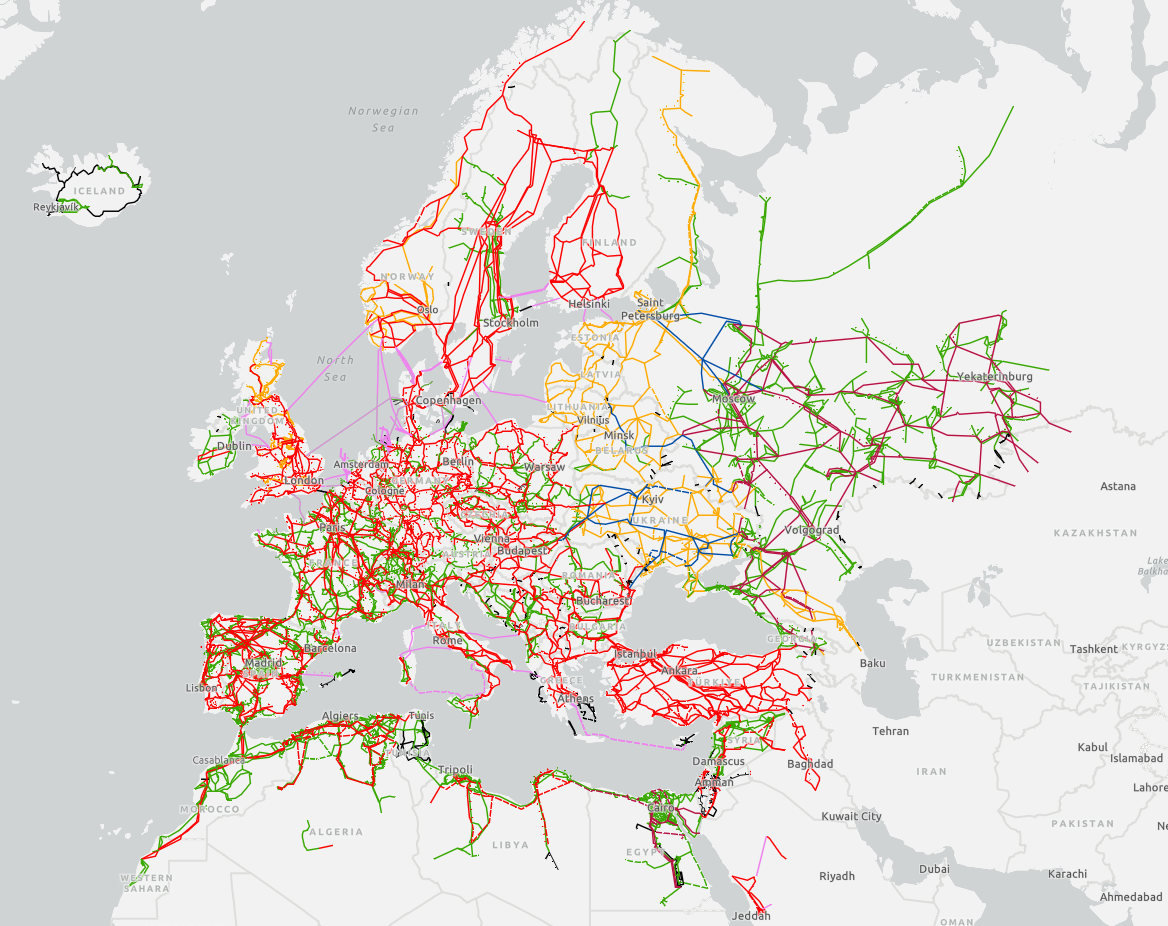
\includegraphics[width=0.68\textwidth]{chapter5pics/hvdcMap.png}
                \caption{Grid map of Europe, with HVDC links in purple.}
                \label{fig:hvdcMap}
            \end{figure}
        \end{column}
    \end{columns}
\end{frame}


% \subsection{Objectives}
\begin{frame}{Objectives}
    \begin{columns}
        % Left column with the image of GridCal
        \begin{column}{0.6\textwidth}
            \begin{figure}[H]
                \centering
                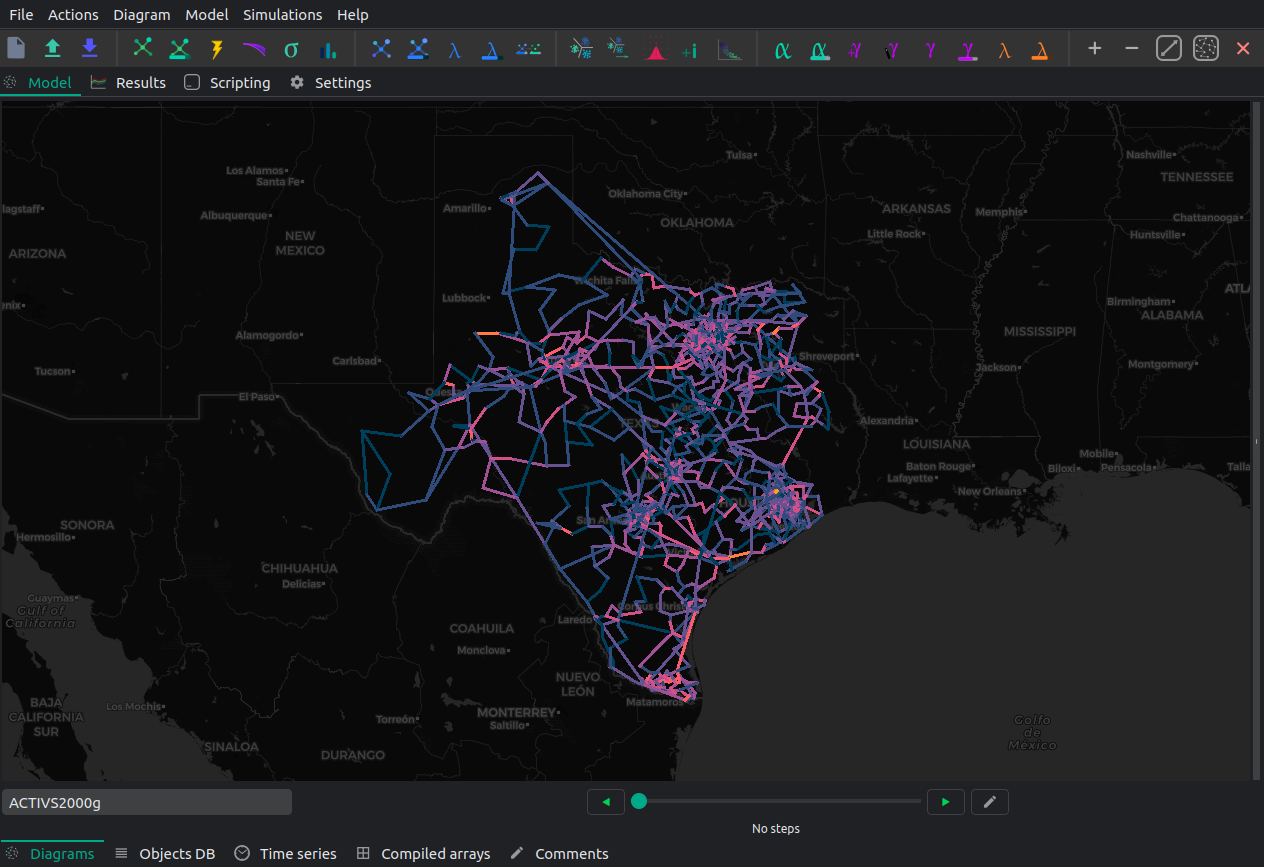
\includegraphics[width=0.95\textwidth]{chapter5pics/gridcalUI.png}
                \caption{GridCal interface used for power flow analysis in Spain.}
                \label{fig:gridcal_interface}
            \end{figure}
        \end{column}
        
        % Right column with the bullet points
        \begin{column}{0.4\textwidth}
            \begin{itemize}
                \item Integrate both AC and DC systems into a unified framework.
                \item Address the convergence issues found in current methods.
                \item Model complex components like converters and controllable transformers.
                \item Implement the method and test its scalability.
            \end{itemize}
        \end{column}
    \end{columns}
\end{frame}


% Include the comparison table after the Generalized Power Flow slide
\begin{frame}{Comparison of features}
    We present a generalised approach to the power flow problem, much more flexible than conventional methods.
    
    \begin{table}[htbp]
    \centering
    \begin{tabular}{|l|c|c|c|}
    \hline
    \textbf{Feature} & \textbf{Traditional} & \textbf{Classical} & \textbf{Generalised} \\ \hline
    Handles AC systems & \(\checkmark\) & \(\checkmark\) & \(\checkmark\) \\ \hline
    Remote controls & \(\times\) & \(\times\) & \(\checkmark\) \\ \hline
    Control more than two magnitudes at a bus & \(\times\) & \(\checkmark\) & \(\checkmark\) \\ \hline
    Controlled branch magnitudes & \(\times\) & \(\checkmark\) & \(\checkmark\) \\ \hline
    Interconnected AC/DC grids & \(\times\) & \(\checkmark\) & \(\checkmark\) \\ \hline
    Flexible bus type definition & \(\times\) & \(\times\) & \(\checkmark\) \\ \hline
    \end{tabular}
    \caption{Comparison between traditional, classical, and generalised power flow.}
    \label{tab:generalisedPfFeatures}
    \end{table}
\end{frame}







% 2. Theory, say something on grid of grids
\section{AC/DC theory}

\begin{frame}{}
    \tableofcontents[currentsection]
\end{frame}

\subsection{Grid basics}
\begin{frame}{What is a power grid?}

\begin{figure}[!htb]
    \centering
    \begin{tikzpicture}[european, scale=0.9]

        % 0. Draw nodes
        \node(1) at (-0.2, 0) {1};
        \node(2) at (1.8, -2) {2};
        \node(3) at (5.0, -2) {3};
        \node(4) at (5.8, 0) {4};
        \node(5) at (4.0, 0) {5};
        \node(6) at (4.0, 1.5) {6};

        % 1. Draw buses (Passive lines in blue)
        \draw[line width=0.1cm] (0, 0) to [short] (0.8, 0);
        \draw[line width=0.1cm] (2, -2) to [short] (2.8, -2);
        \draw[line width=0.1cm] (6, 0) to [short] (6.8, 0);
        \draw[line width=0.1cm] (3, 0) to [short] (3.8, 0);
        \draw[line width=0.1cm] (4, -2) to [short] (4.8, -2);
        \draw[line width=0.1cm] (3, 1.5) to [short] (3.8, 1.5);

        % 2. Draw transformers (red circles)
        \draw[thick, black] (3.4, 0.65) circle (0.2cm);
        \draw[thick, black] (3.4, 0.85) circle (0.2cm);

        % 3. Draw generators with additional busbars
        \draw (0.4, 0.75) to [/tikz/circuitikz/bipoles/length=25pt, sinusoidal voltage source] (0.4, 0.25);
        \draw (0.4, 0.25) to [short] (0.4, 0); 

        \draw (2.4, -2.25) to [/tikz/circuitikz/bipoles/length=25pt, sinusoidal voltage source] (2.4, -2.75);
        \draw (2.4, -2.25) to [short] (2.4, -2.0); 

        \draw (4.4, -2.25) to [/tikz/circuitikz/bipoles/length=25pt, sinusoidal voltage source] (4.4, -2.75);
        \draw (4.4, -2.25) to [short] (4.4, -2.0); 

        % 4. Draw loads
        \draw (2.1, -2) to [short] (2.1, -2.2);
        \draw[-{Latex[scale=1.5]}] (2.1,-2.2) -- (1.3,-2.2);

        \draw (4.7, -2) to [short] (4.7, -2.2);
        \draw[-{Latex[scale=1.5]}] (4.7,-2.2) -- (5.5,-2.2);

        \draw (6.8, 0) to [short] (7.0, 0);
        \draw[-{Latex[scale=1.5]}] (7.0, 0) -- (7.0, -0.8);

        \draw (3.1, 0) to [short] (3.1, 0.2);
        \draw[-{Latex[scale=1.5]}] (3.1, 0.2) -- (2.3, 0.2);

        \draw (3.7, 1.5) to [short] (3.7, 1.7);
        \draw[-{Latex[scale=1.5]}] (3.7, 1.7) -- (4.5, 1.7);

        % Draw lines (Passive lines in blue)
        \draw[black] (0.4, 0) to [short] (0.4, -0.2);
        \draw[black] (2.2, -2) to [short] (2.2, -1.8);
        \draw[black] (0.4, -0.2) to [short] (2.2, -1.8);

        \draw[black] (0.6, 0) to [short] (0.6, -0.2);
        \draw[black] (3.2, 0) to [short] (3.2, -0.2);
        \draw[black] (0.6, -0.2) to [short] (3.2, -0.2);

        \draw[black] (3.4, 0) to [short] (3.4, -0.2);
        \draw[black] (2.4, -2) to [short] (2.4, -1.8);
        \draw[black] (3.4, -0.2) to [short] (2.4, -1.8);

        \draw[black] (2.6, -2) to [short] (2.6, -2.2);
        \draw[black] (4.2, -2) to [short] (4.2, -2.2);
        \draw[black] (2.6, -2.2) to [short] (4.2, -2.2);

        \draw[black] (2.6, -2) to [short] (2.6, -1.8);
        \draw[black] (6.4, 0) to [short] (6.4, -0.2);
        \draw[black] (2.6, -1.8) to [short] (6.4, -0.2);

        \draw[black] (3.6, 0) to [short] (3.6, -0.2);
        \draw[black] (6.2, 0) to [short] (6.2, -0.2);
        \draw[black] (3.6, -0.2) to [short] (6.2, -0.2);

        \draw[black] (4.4, -2) to [short] (4.4, -1.8);
        \draw[black] (6.6, 0) to [short] (6.6, -0.2);
        \draw[black] (4.4, -1.8) to [short] (6.6, -0.2);

        \draw[black] (3.4, 0) to [short] (3.4, 0.45);
        \draw[black] (3.4, 1.05) to [short] (3.4, 1.5);
    \end{tikzpicture}
    \caption{Example grid showing buses linked through branches.}
    \label{fig:14bus}
\end{figure}

    A grid is modeled as an undirected graph the set of buses (nodes) are connected to each other by the set of branches (edges):
    \begin{itemize}
        \item \textbf{Buses}: Represent the points in the network where generation, load, or interconnections occur.
        \item \textbf{Branches}: Power lines, transformers and converters, which can be passive or controllable.
    \end{itemize}
\end{frame}



\begin{frame}{Grid of grids}
    \begin{figure}[H]
    \centering
    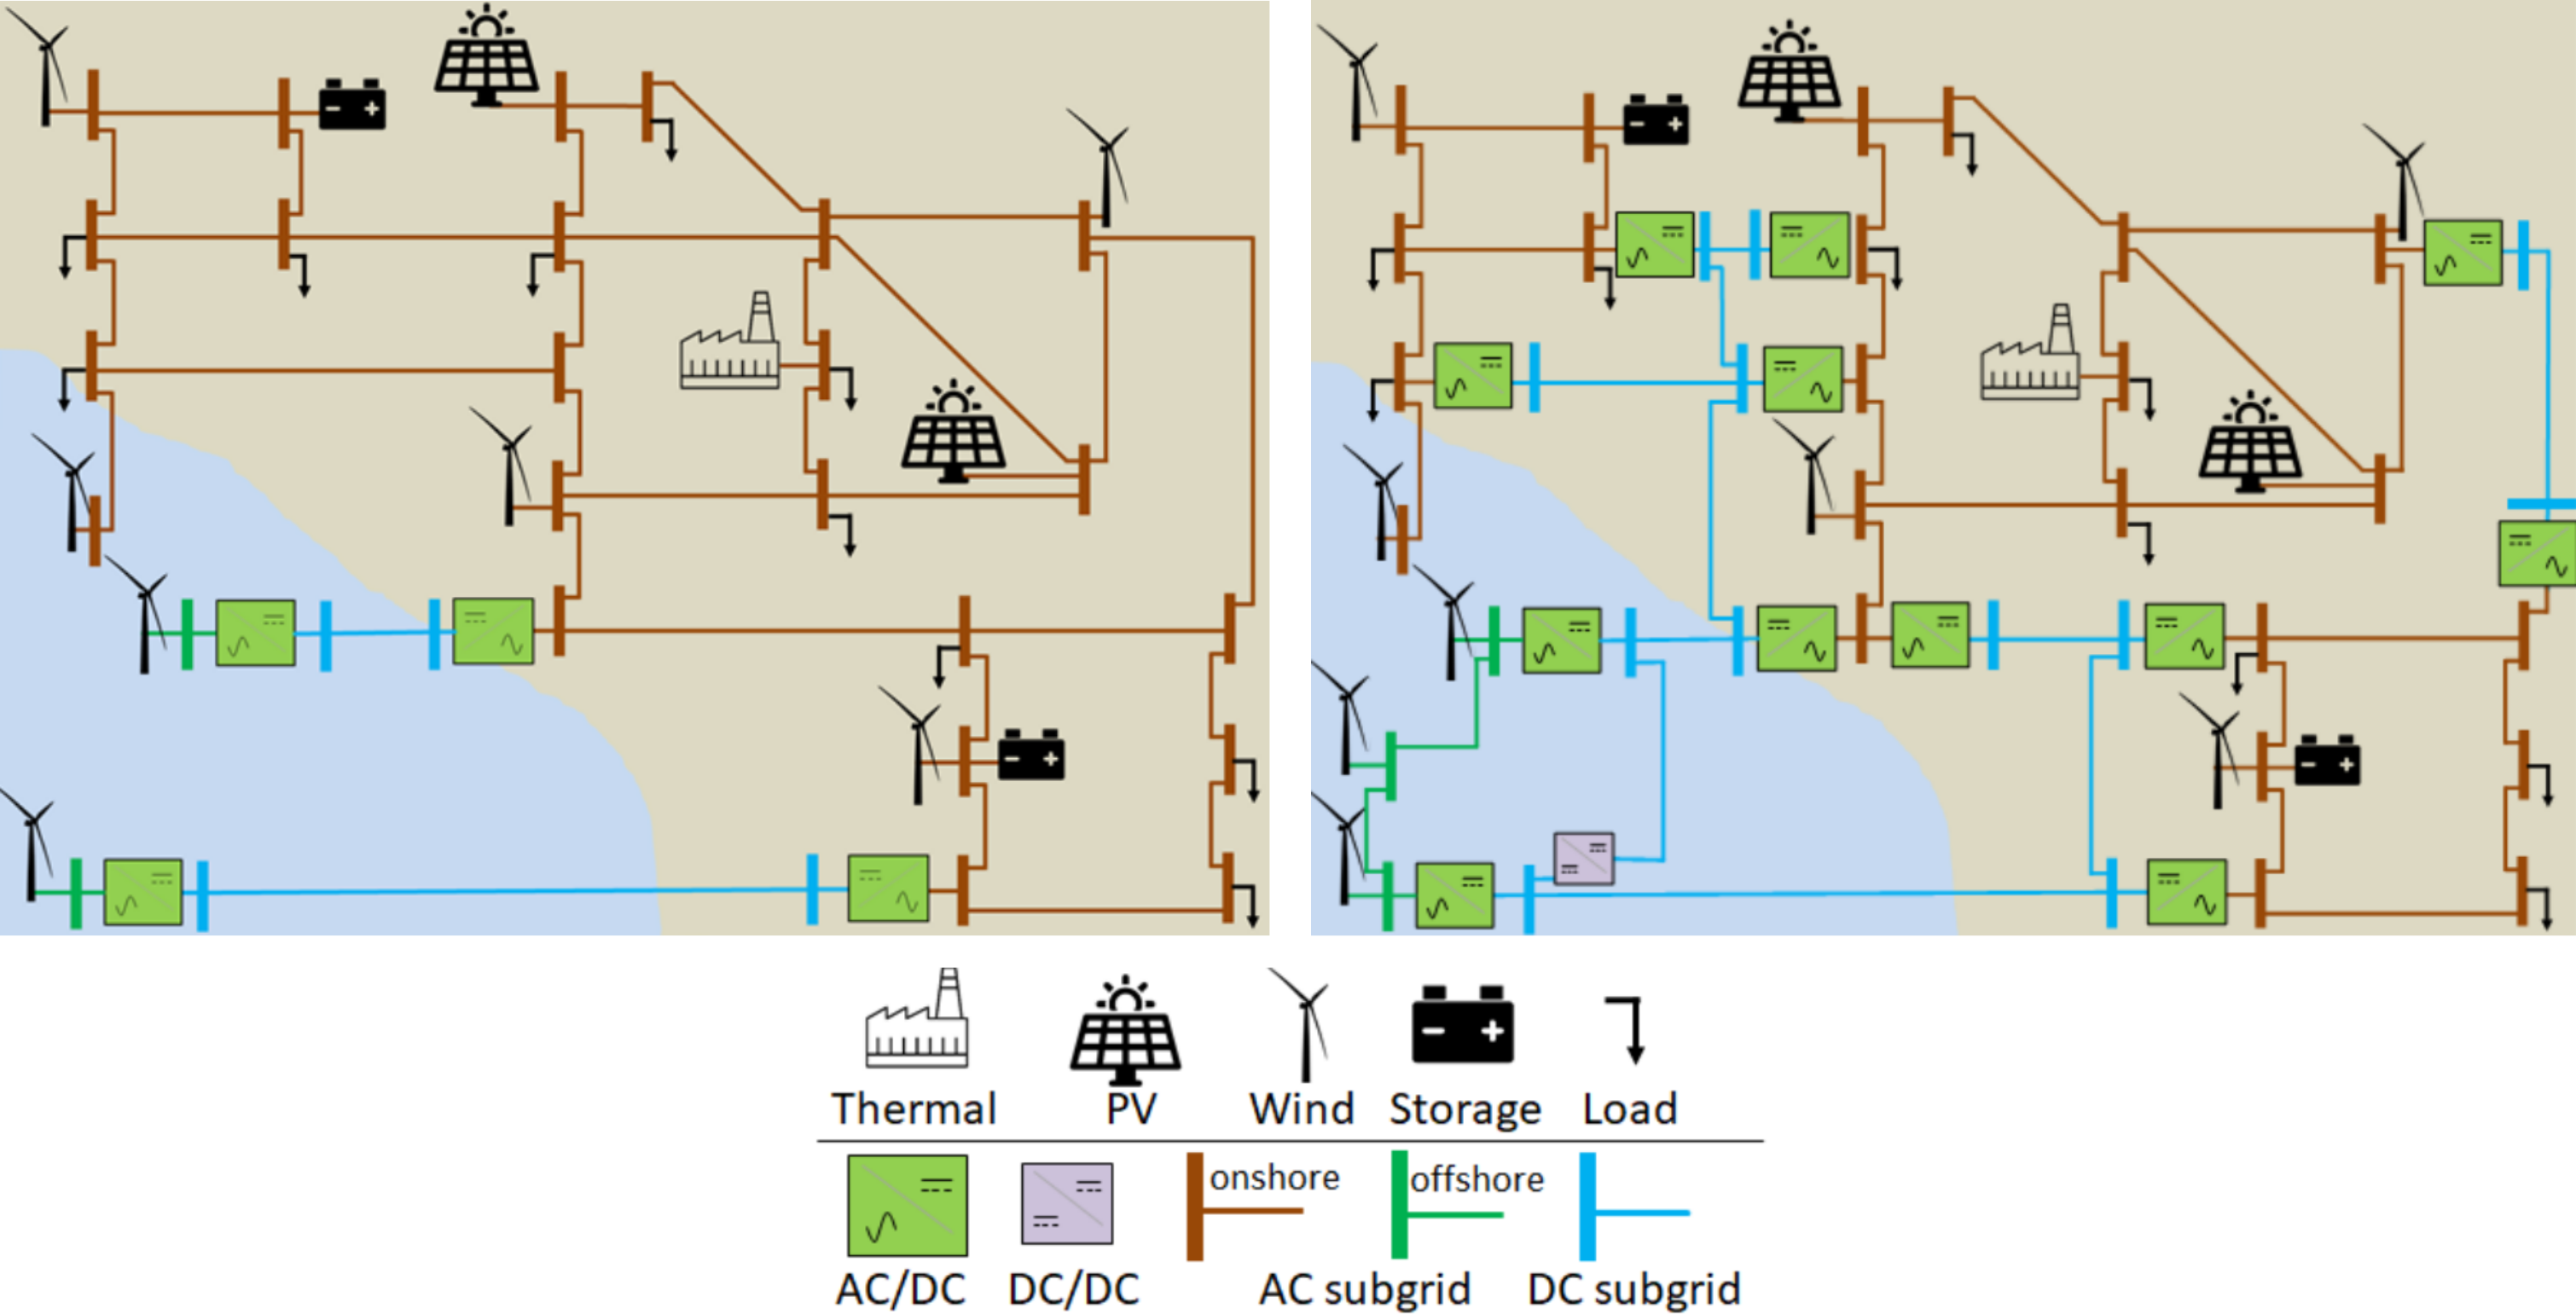
\includegraphics[width=0.9\textwidth]{Images/gridofgrids.png} 
    \caption{From present grids to future systems.}
    \label{fig:gridofgrids}
    \end{figure}
\end{frame}

\subsection{AC/DC converters}
\begin{frame}{Voltage Source Converter (VSC)}
    Voltage source converters (VSCs) interlink AC subsystems with DC subsystems, allowing for controlling two magnitudes. This controllability, while providing more flexibility, also introduces more complexity.
    
    \begin{figure}[!htb]
        \centering
        \begin{circuitikz}[american]
            \draw[line width=0.7mm] (2,0) to [short] (2,-3);
            \draw[line width=0.7mm] (7,0) to [short] (7,-3);
            \draw (2,-1.5) to [sacdc] (7,-1.5);
            \draw (2,-1.5) to [short, i_=$P_t+jQ_t$] (4,-1.5);
            \draw (7,-1.5) to [short, i=$P_f$] (5,-1.5);
            \node at (2,0.35) {$V_t \angle \delta_t$};
            \node at (7,0.35) {$V_f$};
        \end{circuitikz}     
        \caption{Representation of a VSC.}
    \end{figure}
\end{frame}

\begin{frame}{VSC unification of AC and DC sides}
    Converters interconnect DC and AC buses. Hence, there are two approaches to the problem:
    \begin{itemize}
        \item \textbf{Sequential}: we first solve the AC networks, then the DC networks, merge them, and repeat the calculation $\rightarrow$ non-scalable
        \item \textbf{Unified}: we solve all AC and DC grids at the same time $\rightarrow$ much more scalable
    \end{itemize}

    The active powers on the $f$ and $t$ sides are related through the power loss equation:
    \begin{equation}
    \begin{aligned}
        P_f + P_t &= P_{\text{loss}}, \\
        P_f + P_t &= a + b \frac{\sqrt{(P_t)^2 + (Q_t)^2}}{V_t} + c \frac{(P_t)^2 + (Q_t)^2}{V_t^2}. \\
    \end{aligned}
    \end{equation}
\end{frame}


% \subsection{Generalised Branch Model}
% \begin{frame}{Generalised Branch Model}
% \begin{figure}[!htb]
%     \centering
%     \begin{tikzpicture}[european, scale=0.9]

%         % 0. Draw nodes
%         \node(1) at (-0.2, 0) {1};
%         \node(2) at (1.8, -2) {2};
%         \node(3) at (5.0, -2) {3};
%         \node(4) at (5.8, 0) {4};
%         \node(5) at (4.0, 0) {5};
%         \node(6) at (4.0, 1.5) {6};

%         % 1. Draw buses (Passive lines in blue)
%         \draw[line width=0.1cm] (0, 0) to [short] (0.8, 0);
%         \draw[line width=0.1cm] (2, -2) to [short] (2.8, -2);
%         \draw[line width=0.1cm] (6, 0) to [short] (6.8, 0);
%         \draw[line width=0.1cm] (3, 0) to [short] (3.8, 0);
%         \draw[line width=0.1cm] (4, -2) to [short] (4.8, -2);
%         \draw[line width=0.1cm] (3, 1.5) to [short] (3.8, 1.5);

%         % 2. Draw transformers (red circles)
%         \draw[thick, red] (3.4, 0.65) circle (0.2cm);
%         \draw[thick, red] (3.4, 0.85) circle (0.2cm);

%         % 3. Draw generators with additional busbars
%         \draw (0.4, 0.75) to [/tikz/circuitikz/bipoles/length=25pt, sinusoidal voltage source] (0.4, 0.25);
%         \draw (0.4, 0.25) to [short] (0.4, 0); 

%         \draw (2.4, -2.25) to [/tikz/circuitikz/bipoles/length=25pt, sinusoidal voltage source] (2.4, -2.75);
%         \draw (2.4, -2.25) to [short] (2.4, -2.0); 

%         \draw (4.4, -2.25) to [/tikz/circuitikz/bipoles/length=25pt, sinusoidal voltage source] (4.4, -2.75);
%         \draw (4.4, -2.25) to [short] (4.4, -2.0); 

%         % 4. Draw loads
%         \draw (2.1, -2) to [short] (2.1, -2.2);
%         \draw[-{Latex[scale=1.5]}] (2.1,-2.2) -- (1.3,-2.2);

%         \draw (4.7, -2) to [short] (4.7, -2.2);
%         \draw[-{Latex[scale=1.5]}] (4.7,-2.2) -- (5.5,-2.2);

%         \draw (6.8, 0) to [short] (7.0, 0);
%         \draw[-{Latex[scale=1.5]}] (7.0, 0) -- (7.0, -0.8);

%         \draw (3.1, 0) to [short] (3.1, 0.2);
%         \draw[-{Latex[scale=1.5]}] (3.1, 0.2) -- (2.3, 0.2);

%         \draw (3.7, 1.5) to [short] (3.7, 1.7);
%         \draw[-{Latex[scale=1.5]}] (3.7, 1.7) -- (4.5, 1.7);

%         % Draw lines (Passive lines in blue)
%         \draw[blue] (0.4, 0) to [short] (0.4, -0.2);
%         \draw[blue] (2.2, -2) to [short] (2.2, -1.8);
%         \draw[blue] (0.4, -0.2) to [short] (2.2, -1.8);

%         \draw[blue] (0.6, 0) to [short] (0.6, -0.2);
%         \draw[blue] (3.2, 0) to [short] (3.2, -0.2);
%         \draw[blue] (0.6, -0.2) to [short] (3.2, -0.2);

%         \draw[blue] (3.4, 0) to [short] (3.4, -0.2);
%         \draw[blue] (2.4, -2) to [short] (2.4, -1.8);
%         \draw[blue] (3.4, -0.2) to [short] (2.4, -1.8);

%         \draw[blue] (2.6, -2) to [short] (2.6, -2.2);
%         \draw[blue] (4.2, -2) to [short] (4.2, -2.2);
%         \draw[blue] (2.6, -2.2) to [short] (4.2, -2.2);

%         \draw[blue] (2.6, -2) to [short] (2.6, -1.8);
%         \draw[blue] (6.4, 0) to [short] (6.4, -0.2);
%         \draw[blue] (2.6, -1.8) to [short] (6.4, -0.2);

%         \draw[blue] (3.6, 0) to [short] (3.6, -0.2);
%         \draw[blue] (6.2, 0) to [short] (6.2, -0.2);
%         \draw[blue] (3.6, -0.2) to [short] (6.2, -0.2);

%         \draw[blue] (4.4, -2) to [short] (4.4, -1.8);
%         \draw[blue] (6.6, 0) to [short] (6.6, -0.2);
%         \draw[blue] (4.4, -1.8) to [short] (6.6, -0.2);

%         \draw[red] (3.4, 0) to [short] (3.4, 0.45);
%         \draw[red] (3.4, 1.05) to [short] (3.4, 1.5);
%     \end{tikzpicture}
%     \caption{Example grid showing passive lines and active controllable transformer.}
%     \label{fig:14bus}
% \end{figure}



%     In our formulation, we define two sets of branches:
%     \begin{itemize}
%         \item $\kappa$: Passive branches (e.g., lines, non-controllable transformers).
%         \item $\Gamma$: Active branches (e.g., AC/DC interfaces, controllable transformers).
%     \end{itemize}
%     Passive branches ($\kappa$) are reduced to admittances and included in the $Y_\text{bus}$ matrix. Active branches ($\Gamma$) are modeled by power flows through their terminals.
% \end{frame}


% \begin{frame}{Passive Branches}
%     \begin{figure}[!htb]
%         \centering
%         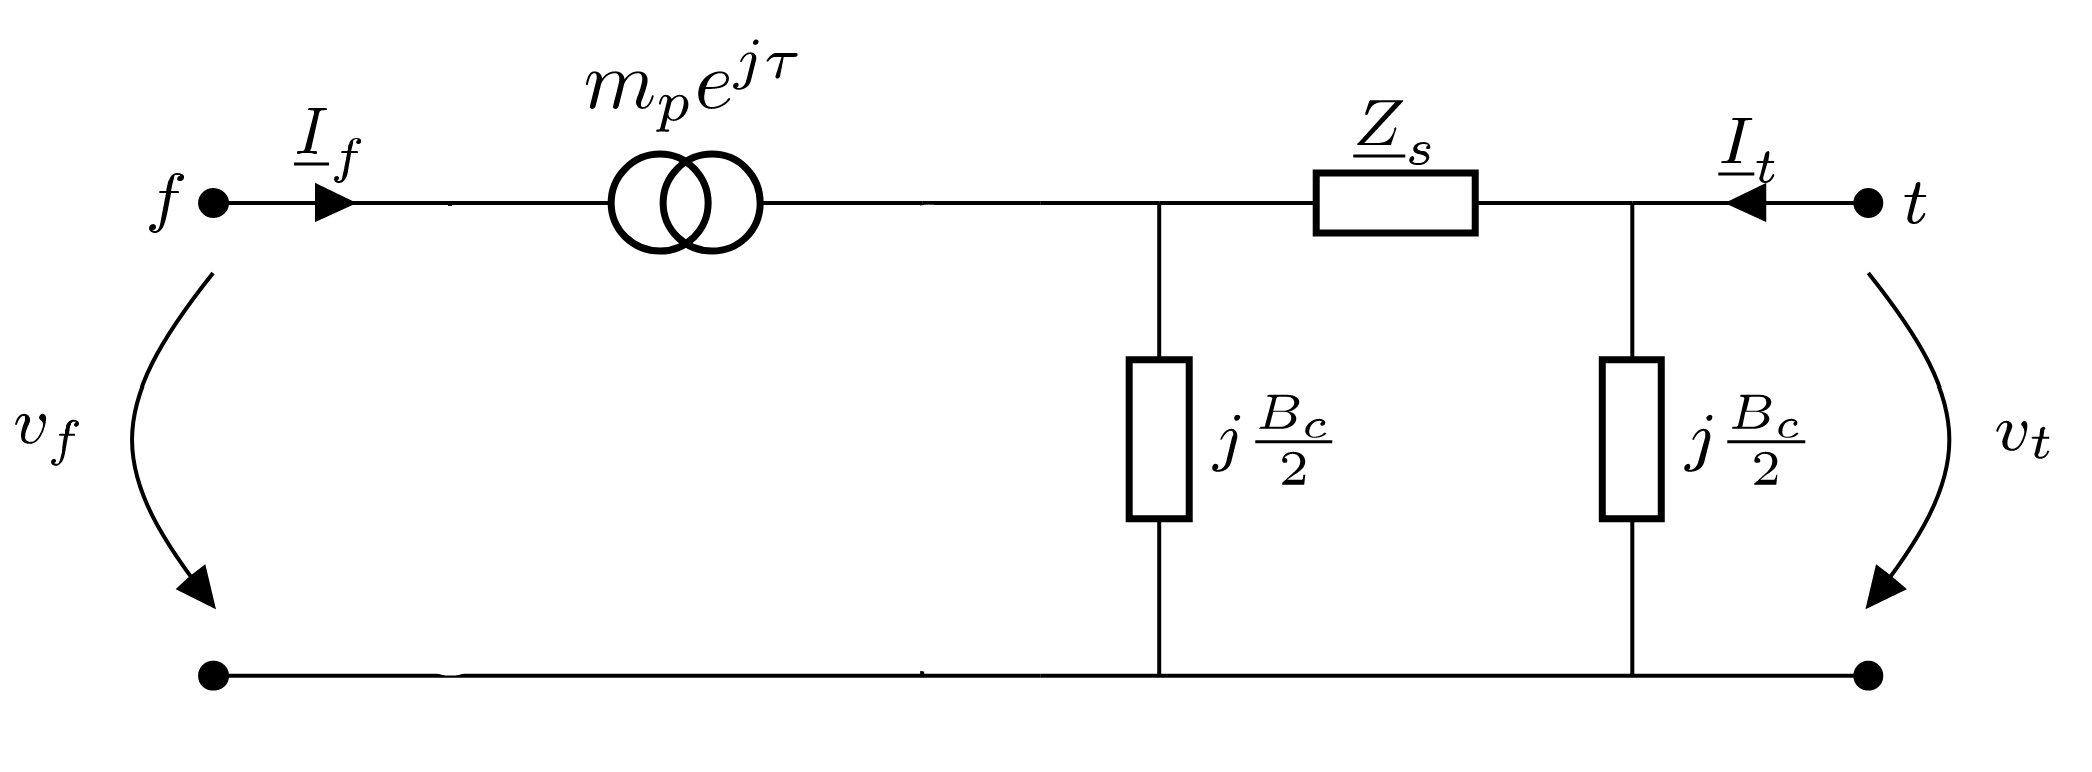
\includegraphics[width=0.6\textwidth]{chapter5pics/branch.png}
%         \caption{Representation of a passive branch.}
%         \label{fig:FUBM}
%     \end{figure} 


%     For any branch $b \in \kappa$ (passive branches), you have a two-by-two admittance matrix:
%     \[
%         Y_{b\in\kappa} = 
%         \begin{bmatrix}
%             Y_{ff} & Y_{ft} \\
%             Y_{tf} & Y_{tt}
%         \end{bmatrix}
%     \]
%     where $Y_{ff}$, $Y_{ft}$, $Y_{tf}$, and $Y_{tt}$ represent the admittance values from the \textit{from} ($f$) and \textit{to} ($t$) sides. The system's $Y_\text{bus}$ matrix is constructed by combining the admittance contributions of all passive branches connected to each bus in the network.
% \end{frame}

% \begin{frame}{FUBM}
%     \begin{figure}[!htb]
%         \centering
%         \includesvg[width=0.6\textwidth]{Images/FUBM.svg}
%         \caption{Flexible Universal Branch Model.}
%         \label{fig:FUBM}
%     \end{figure} 
% The idea of the FUBM is to represent various components in power systems (transmission lines, transformers, and VSCs) in a standardised manner. This model makes no distinction between active and passive branches.

% \end{frame}


% \section{Solving } 

% \begin{frame}{}
%     \tableofcontents[currentsection]
% \end{frame}

\subsection{The power flow}
\begin{frame}{The power flow problem}
    \begin{itemize}
        \item Grid operators are interested in knowing the operating state of the network.
        \item That is, voltages, currents and powers have to be found everywhere in the grid.
        \item The underlying equations, which come from the physics, are non-linear in nature.
        \item Among many solvers, we opt for the Newton-Raphson given its quadratic convergence and scalability properties.
    \end{itemize}

    \begin{equation}
    \bm{x} = [\delta, V, \textcolor{red}{\tau}, \textcolor{red}{m}, \textcolor{red}{P^\text{zip}}, \textcolor{red}{Q^\text{zip}}, \textcolor{red}{P_f}, \textcolor{red}{P_t}, \textcolor{red}{Q_f}, \textcolor{red}{Q_t}]^T
    \end{equation}
    \begin{equation}
    \mathbf{g} =
    [g_{p,ac}, g_{q,ac}, g_{p,dc}, \textcolor{red}{g_{l,acdc}}, \textcolor{red}{g_{l,hvdc}}, \textcolor{red}{g_{p,hvdc}}, \textcolor{red}{g_{p_f,tr}}, \textcolor{red}{g_{p_t,tr}}, \textcolor{red}{g_{q_f,tr}}, \textcolor{red}{g_{q_t,tr}}]^T
    \end{equation}
\end{frame}

\subsection{Solving approach}
\begin{frame}{The Newton-Raphson method}
    \begin{itemize}
    \item To solve the system using the Newton-Raphson method, we need a Jacobian matrix. 
    
    \item This matrix contains the partial derivatives of the form $\frac{\partial{\bm{g}}}{\partial{\bm{x}}}$. Two ways to calculate:
    \begin{enumerate}
        \item Partial differences such as $\frac{\bm{g}(\bm{x} + h) - \bm{g}(\bm{x} - h)}{h}$ $\rightarrow$ easier but slower
        \item With previously derived closed-form expressions $\rightarrow$ harder but faster
    \end{enumerate}
    
    \item The typical Newton-Raphson system is represented as:
    \end{itemize}

    \begin{equation}
        -\mathbf{J} \Delta \mathbf{x} = \mathbf{g}
    \end{equation}
    where:
    \begin{itemize}
        \item $\mathbf{J}$ is the Jacobian matrix.
        \item $\Delta \mathbf{x}$ is the vector of unknown variations.
        \item $\mathbf{g}$ is the residual vector of equations.
    \end{itemize}
\end{frame}

% \begin{frame}{Solving Generalized Power Flow with Newton-Raphson}
%     To solve the generalized power flow problem, a set of known and unknown magnitudes must be defined. 
%     \begin{itemize}
%         \item Known magnitudes are those actively controlled by the system.
%         \item Unknown magnitudes are not directly controlled.
%     \end{itemize}
%     The unknown set $x$ includes:
% \[
% x = [\delta, V, \textcolor{red}{\tau}, \textcolor{red}{m}, \textcolor{red}{P^\text{zip}}, \textcolor{red}{Q^\text{zip}}, \textcolor{red}{P_f}, \textcolor{red}{P_t}, \textcolor{red}{Q_f}, \textcolor{red}{Q_t}]^T
% \]
% \[
% |x| = |\text{DC}|+ 2 \cdot |\text{AC}| + 3 \cdot |\text{VSC}| + 4 \cdot |\text{TR}|
% \]


%     This generalized formulation extends the traditional model by incorporating more unknowns, such as controlled transformers and AC/DC links.
% \end{frame}

% \subsection{Equations and Nodal Balance}
% \begin{frame}{Equations and Nodal Balance (1)}
%     The system of equations must balance the number of unknowns and equations. The nodal balance equations include:
%     \begin{itemize}
%         \item Nodal active and reactive power at AC buses.
%         \item Active power at DC buses.
%         \item Power loss equations for AC/DC links.
%         \item Power equations for controlled transformers.
%         \item Power equations for remotely-controlled passive branches.
%     \end{itemize}
% \end{frame}

% \begin{frame}{Jacobian Variables}
%     The unknown vector $\Delta \mathbf{x}$ is represented as:
%     \[
%     \Delta \mathbf{x} =
%     [\Delta \delta, \Delta V, \Delta \tau, \Delta m, \Delta P^\text{zip}, \Delta Q^\text{zip}, \Delta P_f, \Delta P_t, \Delta Q_f, \Delta Q_t]^T
%     \]
%     The residual vector $\mathbf{g}$ is:
%     \[
%     \mathbf{g} =
%     [g_{p,ac}, g_{q,ac}, g_{p,dc}, g_{p,acdc}, g_{p_f,tr}, g_{p_t,tr}, g_{q_f,tr}, g_{q_t,tr}, g_{p_{ij}, \kappa}, g_{q_{ij}, \kappa}, g_{p_{ji}, \kappa}, g_{q_{ji}, \kappa}]^T
%     \]
% \end{frame}


% \begin{frame}{Jacobian Matrix in Full}
%     \scriptsize  % Shrinks the font size to make it fit better on the slide
%     The full Jacobian matrix $\mathbf{J}$ is constructed as follows, showing the partial derivatives of the equations with respect to the unknown variables:
    
%     \[
%     \mathbf{J} = 
%     \begin{bmatrix}
%         \frac{\partial g_{p,ac}}{\partial \delta} & \frac{\partial g_{p,ac}}{\partial V} & \frac{\partial g_{p,ac}}{\partial \tau} & \frac{\partial g_{p,ac}}{\partial m} & \frac{\partial g_{p,ac}}{\partial P^\text{zip}} & \frac{\partial g_{p,ac}}{\partial Q^\text{zip}} & \frac{\partial g_{p,ac}}{\partial P_f} & \frac{\partial g_{p,ac}}{\partial P_t} & \frac{\partial g_{p,ac}}{\partial Q_f} & \frac{\partial g_{p,ac}}{\partial Q_t} \\
%         \frac{\partial g_{q,ac}}{\partial \delta} & \frac{\partial g_{q,ac}}{\partial V} & \frac{\partial g_{q,ac}}{\partial \tau} & \frac{\partial g_{q,ac}}{\partial m} & \frac{\partial g_{q,ac}}{\partial P^\text{zip}} & \frac{\partial g_{q,ac}}{\partial Q^\text{zip}} & \frac{\partial g_{q,ac}}{\partial P_f} & \frac{\partial g_{q,ac}}{\partial P_t} & \frac{\partial g_{q,ac}}{\partial Q_f} & \frac{\partial g_{q,ac}}{\partial Q_t} \\
%         \frac{\partial g_{p,dc}}{\partial \delta} & \frac{\partial g_{p,dc}}{\partial V} & \frac{\partial g_{p,dc}}{\partial \tau} & \frac{\partial g_{p,dc}}{\partial m} & \frac{\partial g_{p,dc}}{\partial P^\text{zip}} & \frac{\partial g_{p,dc}}{\partial Q^\text{zip}} & \frac{\partial g_{p,dc}}{\partial P_f} & \frac{\partial g_{p,dc}}{\partial P_t} & \frac{\partial g_{p,dc}}{\partial Q_f} & \frac{\partial g_{p,dc}}{\partial Q_t} \\
%         \frac{\partial g_{p,acdc}}{\partial \delta} & \frac{\partial g_{p,acdc}}{\partial V} & \frac{\partial g_{p,acdc}}{\partial \tau} & \frac{\partial g_{p,acdc}}{\partial m} & \frac{\partial g_{p,acdc}}{\partial P^\text{zip}} & \frac{\partial g_{p,acdc}}{\partial Q^\text{zip}} & \frac{\partial g_{p,acdc}}{\partial P_f} & \frac{\partial g_{p,acdc}}{\partial P_t} & \frac{\partial g_{p,acdc}}{\partial Q_f} & \frac{\partial g_{p,acdc}}{\partial Q_t} \\
%         \frac{\partial g_{p_f,tr}}{\partial \delta} & \frac{\partial g_{p_f,tr}}{\partial V} & \frac{\partial g_{p_f,tr}}{\partial \tau} & \frac{\partial g_{p_f,tr}}{\partial m} & \frac{\partial g_{p_f,tr}}{\partial P^\text{zip}} & \frac{\partial g_{p_f,tr}}{\partial Q^\text{zip}} & \frac{\partial g_{p_f,tr}}{\partial P_f} & \frac{\partial g_{p_f,tr}}{\partial P_t} & \frac{\partial g_{p_f,tr}}{\partial Q_f} & \frac{\partial g_{p_f,tr}}{\partial Q_t} \\
%         \frac{\partial g_{p_t,tr}}{\partial \delta} & \frac{\partial g_{p_t,tr}}{\partial V} & \frac{\partial g_{p_t,tr}}{\partial \tau} & \frac{\partial g_{p_t,tr}}{\partial m} & \frac{\partial g_{p_t,tr}}{\partial P^\text{zip}} & \frac{\partial g_{p_t,tr}}{\partial Q^\text{zip}} & \frac{\partial g_{p_t,tr}}{\partial P_f} & \frac{\partial g_{p_t,tr}}{\partial P_t} & \frac{\partial g_{p_t,tr}}{\partial Q_f} & \frac{\partial g_{p_t,tr}}{\partial Q_t} \\
%         \frac{\partial g_{q_f,tr}}{\partial \delta} & \frac{\partial g_{q_f,tr}}{\partial V} & \frac{\partial g_{q_f,tr}}{\partial \tau} & \frac{\partial g_{q_f,tr}}{\partial m} & \frac{\partial g_{q_f,tr}}{\partial P^\text{zip}} & \frac{\partial g_{q_f,tr}}{\partial Q^\text{zip}} & \frac{\partial g_{q_f,tr}}{\partial P_f} & \frac{\partial g_{q_f,tr}}{\partial P_t} & \frac{\partial g_{q_f,tr}}{\partial Q_f} & \frac{\partial g_{q_f,tr}}{\partial Q_t} \\
%         \frac{\partial g_{q_t,tr}}{\partial \delta} & \frac{\partial g_{q_t,tr}}{\partial V} & \frac{\partial g_{q_t,tr}}{\partial \tau} & \frac{\partial g_{q_t,tr}}{\partial m} & \frac{\partial g_{q_t,tr}}{\partial P^\text{zip}} & \frac{\partial g_{q_t,tr}}{\partial Q^\text{zip}} & \frac{\partial g_{q_t,tr}}{\partial P_f} & \frac{\partial g_{q_t,tr}}{\partial P_t} & \frac{\partial g_{q_t,tr}}{\partial Q_f} & \frac{\partial g_{q_t,tr}}{\partial Q_t} \\
%         \frac{\partial g_{pf, \kappa }}{\partial \delta} & \frac{\partial g_{pf, \kappa }}{\partial V} & \frac{\partial g_{pf, \kappa }}{\partial \tau} & \frac{\partial g_{pf, \kappa }}{\partial m} & \frac{\partial g_{pf, \kappa }}{\partial P^\text{zip}} & \frac{\partial g_{pf, \kappa }}{\partial Q^\text{zip}} & \frac{\partial g_{pf, \kappa }}{\partial P_f} & \frac{\partial g_{pf, \kappa }}{\partial P_t} & \frac{\partial g_{pf, \kappa }}{\partial Q_f} & \frac{\partial g_{pf, \kappa }}{\partial Q_t} \\
%         \frac{\partial g_{qf, \kappa }}{\partial \delta} & \frac{\partial g_{qf, \kappa }}{\partial V} & \frac{\partial g_{qf, \kappa }}{\partial \tau} & \frac{\partial g_{qf, \kappa }}{\partial m} & \frac{\partial g_{qf, \kappa }}{\partial P^\text{zip}} & \frac{\partial g_{qf, \kappa }}{\partial Q^\text{zip}} & \frac{\partial g_{qf, \kappa }}{\partial P_f} & \frac{\partial g_{qf, \kappa }}{\partial P_t} & \frac{\partial g_{qf, \kappa }}{\partial Q_f} & \frac{\partial g_{qf, \kappa }}{\partial Q_t} \\
%         \frac{\partial g_{pt, \kappa }}{\partial \delta} & \frac{\partial g_{pt, \kappa }}{\partial V} & \frac{\partial g_{pt, \kappa }}{\partial \tau} & \frac{\partial g_{pt, \kappa }}{\partial m} & \frac{\partial g_{pt, \kappa }}{\partial P^\text{zip}} & \frac{\partial g_{pt, \kappa }}{\partial Q^\text{zip}} & \frac{\partial g_{pt, \kappa }}{\partial P_f} & \frac{\partial g_{pt, \kappa }}{\partial P_t} & \frac{\partial g_{pt, \kappa }}{\partial Q_f} & \frac{\partial g_{pt, \kappa }}{\partial Q_t} \\
%         \frac{\partial g_{qt, \kappa }}{\partial \delta} & \frac{\partial g_{qt, \kappa }}{\partial V} & \frac{\partial g_{qt, \kappa }}{\partial \tau} & \frac{\partial g_{qt, \kappa }}{\partial m} & \frac{\partial g_{qt, \kappa }}{\partial P^\text{zip}} & \frac{\partial g_{qt, \kappa }}{\partial Q^\text{zip}} & \frac{\partial g_{qt, \kappa }}{\partial P_f} & \frac{\partial g_{qt, \kappa }}{\partial P_t} & \frac{\partial g_{qt, \kappa }}{\partial Q_f} & \frac{\partial g_{qt, \kappa }}{\partial Q_t}
%     \end{bmatrix}
%     \]
% \end{frame}




\begin{frame}{Rules for solvability}
    \begin{columns}
        % Left column with the rules
        \begin{column}{0.5\textwidth}
            To ensure solvability in generalized power flow, the following rules are defined:
            \begin{itemize}
                \item Each subgrid must have at least one reference for voltage magnitude and angle.
                \item Control of a remote bus is allowed.
                \item No two devices can control the same nodal voltage.
                \item Buses can have up to 4 controlled magnitudes in AC subsystems and 2 in DC subsystems.
            \end{itemize}
        \end{column}
        
        % Right column with the figure
        \begin{column}{0.5\textwidth}
            \begin{figure}[H]
                \centering
                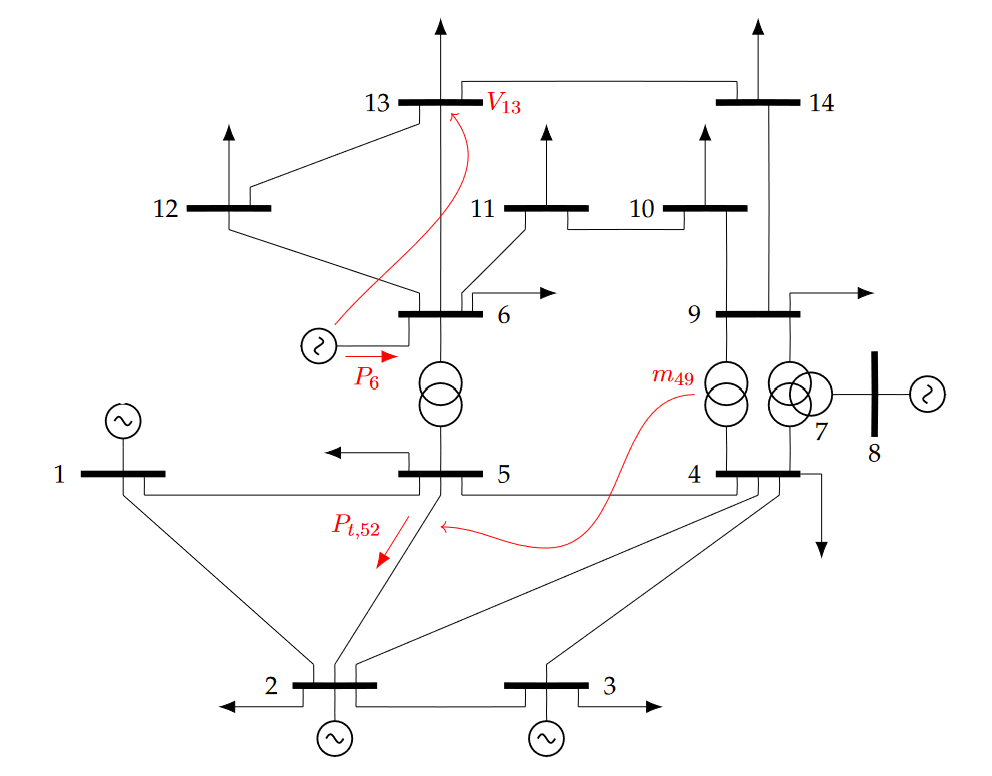
\includegraphics[width=0.9\textwidth]{chapter5pics/remote.png}
                \caption{Scheme of the IEEE 14-bus grid with remote controls.}
                \label{fig:simple6bus}
            \end{figure}
        \end{column}
    \end{columns}
\end{frame}





% 3. Installation
\section{Installation}

\begin{frame}{}
    \tableofcontents[currentsection]
\end{frame}


\begin{frame}{Installation}
    % try it on my own on a second computer
    % try also what happens with Python 3.12 or 3.13
    The three requisites are:
    \begin{enumerate}
        \item Python 3.10 or 3.11.
        \item VSCode.
        \item GridCal wheels.
    \end{enumerate}
\end{frame}

\begin{frame}{Python installation}
    \begin{itemize}
        \item For instance, download Python 3.10.9 from \href{https://www.python.org/downloads/release/python-3109/}{https://www.python.org/downloads/release/python-3109/}.
        \item Make sure to add Python to the PATH.
    \end{itemize}
    \begin{figure}[!htb]
        \centering
        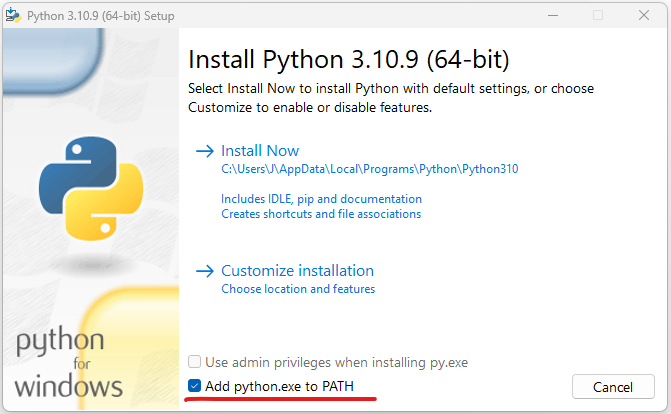
\includegraphics[width=0.6\textwidth]{Images/python_install.png}
        \caption{Python installation.}
        \label{fig:python_installation}
    \end{figure}
\end{frame}

\begin{frame}{VSCode installation}
    \begin{itemize}
        \item Download VSCode from \href{https://code.visualstudio.com/}{https://code.visualstudio.com/}.
        \item Install the Python extension.
    \end{itemize}
        \begin{figure}[!htb]
        \centering
        
\includegraphics[width=0.6\textwidth]{Images/python_vscode.png}
        \caption{Python VSCode extension.}
        \label{fig:vscode_installation}
    \end{figure}
\end{frame}

\begin{frame}{GridCal installation}
    \begin{itemize}
        \item Create a virtual environment in VSCode: Ctrl+Shift+P,  then Python: Create Environment.
        \item Activate with \fbox{"./.venv/Scripts/Activate"}.
        \item Install the latest alpha GridCal release: \fbox{pip install GridCal==5.3.0a1}.
        \item Verify the installation with \fbox{pip list}.
    \end{itemize}
    Open the interface:
    \begin{itemize}
        \item Windows: 
        \begin{center}
            % \fbox{python -c "from GridCal.ExecuteGridCal import run; run()"}
            \fbox{python -c "from GridCal.ExecuteGridCal import runGridCal; runGridCal()"}
        \end{center}
        \item Unix: 
        \begin{center}
            \fbox{python3 -c "from GridCal.ExecuteGridCal import runGridCal; runGridCal()"}
            % \fbox{python3 -c "from GridCal.ExecuteGridCal import run; run()"}
        \end{center}
    \end{itemize}
    % CTRL+SHIFT+P, create virtual env
    % .\.venv\Scripts\Activate
    % pip install GridCal==5.3.0a1
    % https://stackoverflow.com/questions/54776324/powershell-bug-execution-of-scripts-is-disabled-on-this-system
\end{frame}


% 4. Practical (bulk of the work)
\section{Practical cases}

\begin{frame}{}
    \tableofcontents[currentsection]
\end{frame}

% ------------------------------------------
\subsection{Fundamental 6-bus case}
% \begin{frame}{}
%     \tableofcontents[currentsection]
% \end{frame}


\begin{frame}{GUI usage: modelling}
    \fbox{python -c "from GridCal.ExecuteGridCal import runGridCal; runGridCal()"}

    \begin{columns}
        \begin{column}{0.65\textwidth}
    \begin{figure}[H]
        \centering
    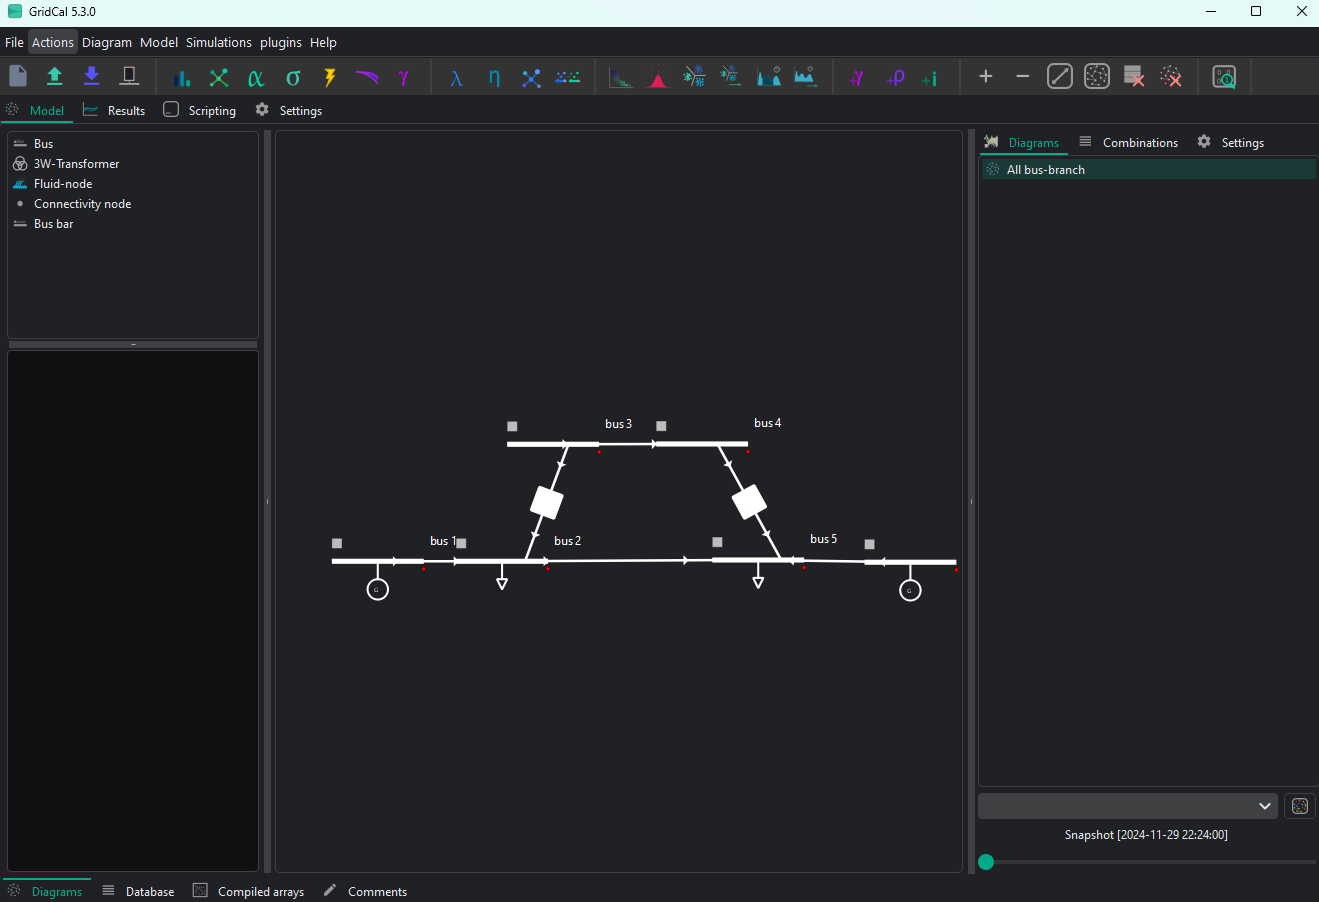
\includegraphics[width=0.99\textwidth]{Images/6busgui.png}
    \caption{Visualization of the 6-bus grid through the GUI.}
    \label{fig:6bus1}
    \end{figure}
        \end{column}
        
        \begin{column}{0.35\textwidth}
            \begin{itemize}
                \item Go over the complete database.
                \item Check the controls of the generators.
                \item Check the controls of the VSCs. What to expect?
            \end{itemize}
        \end{column}
    \end{columns}
\end{frame}

\begin{frame}{GUI usage: solving}
    % solver selection screen and results table
    \begin{figure}[H]
        \centering
    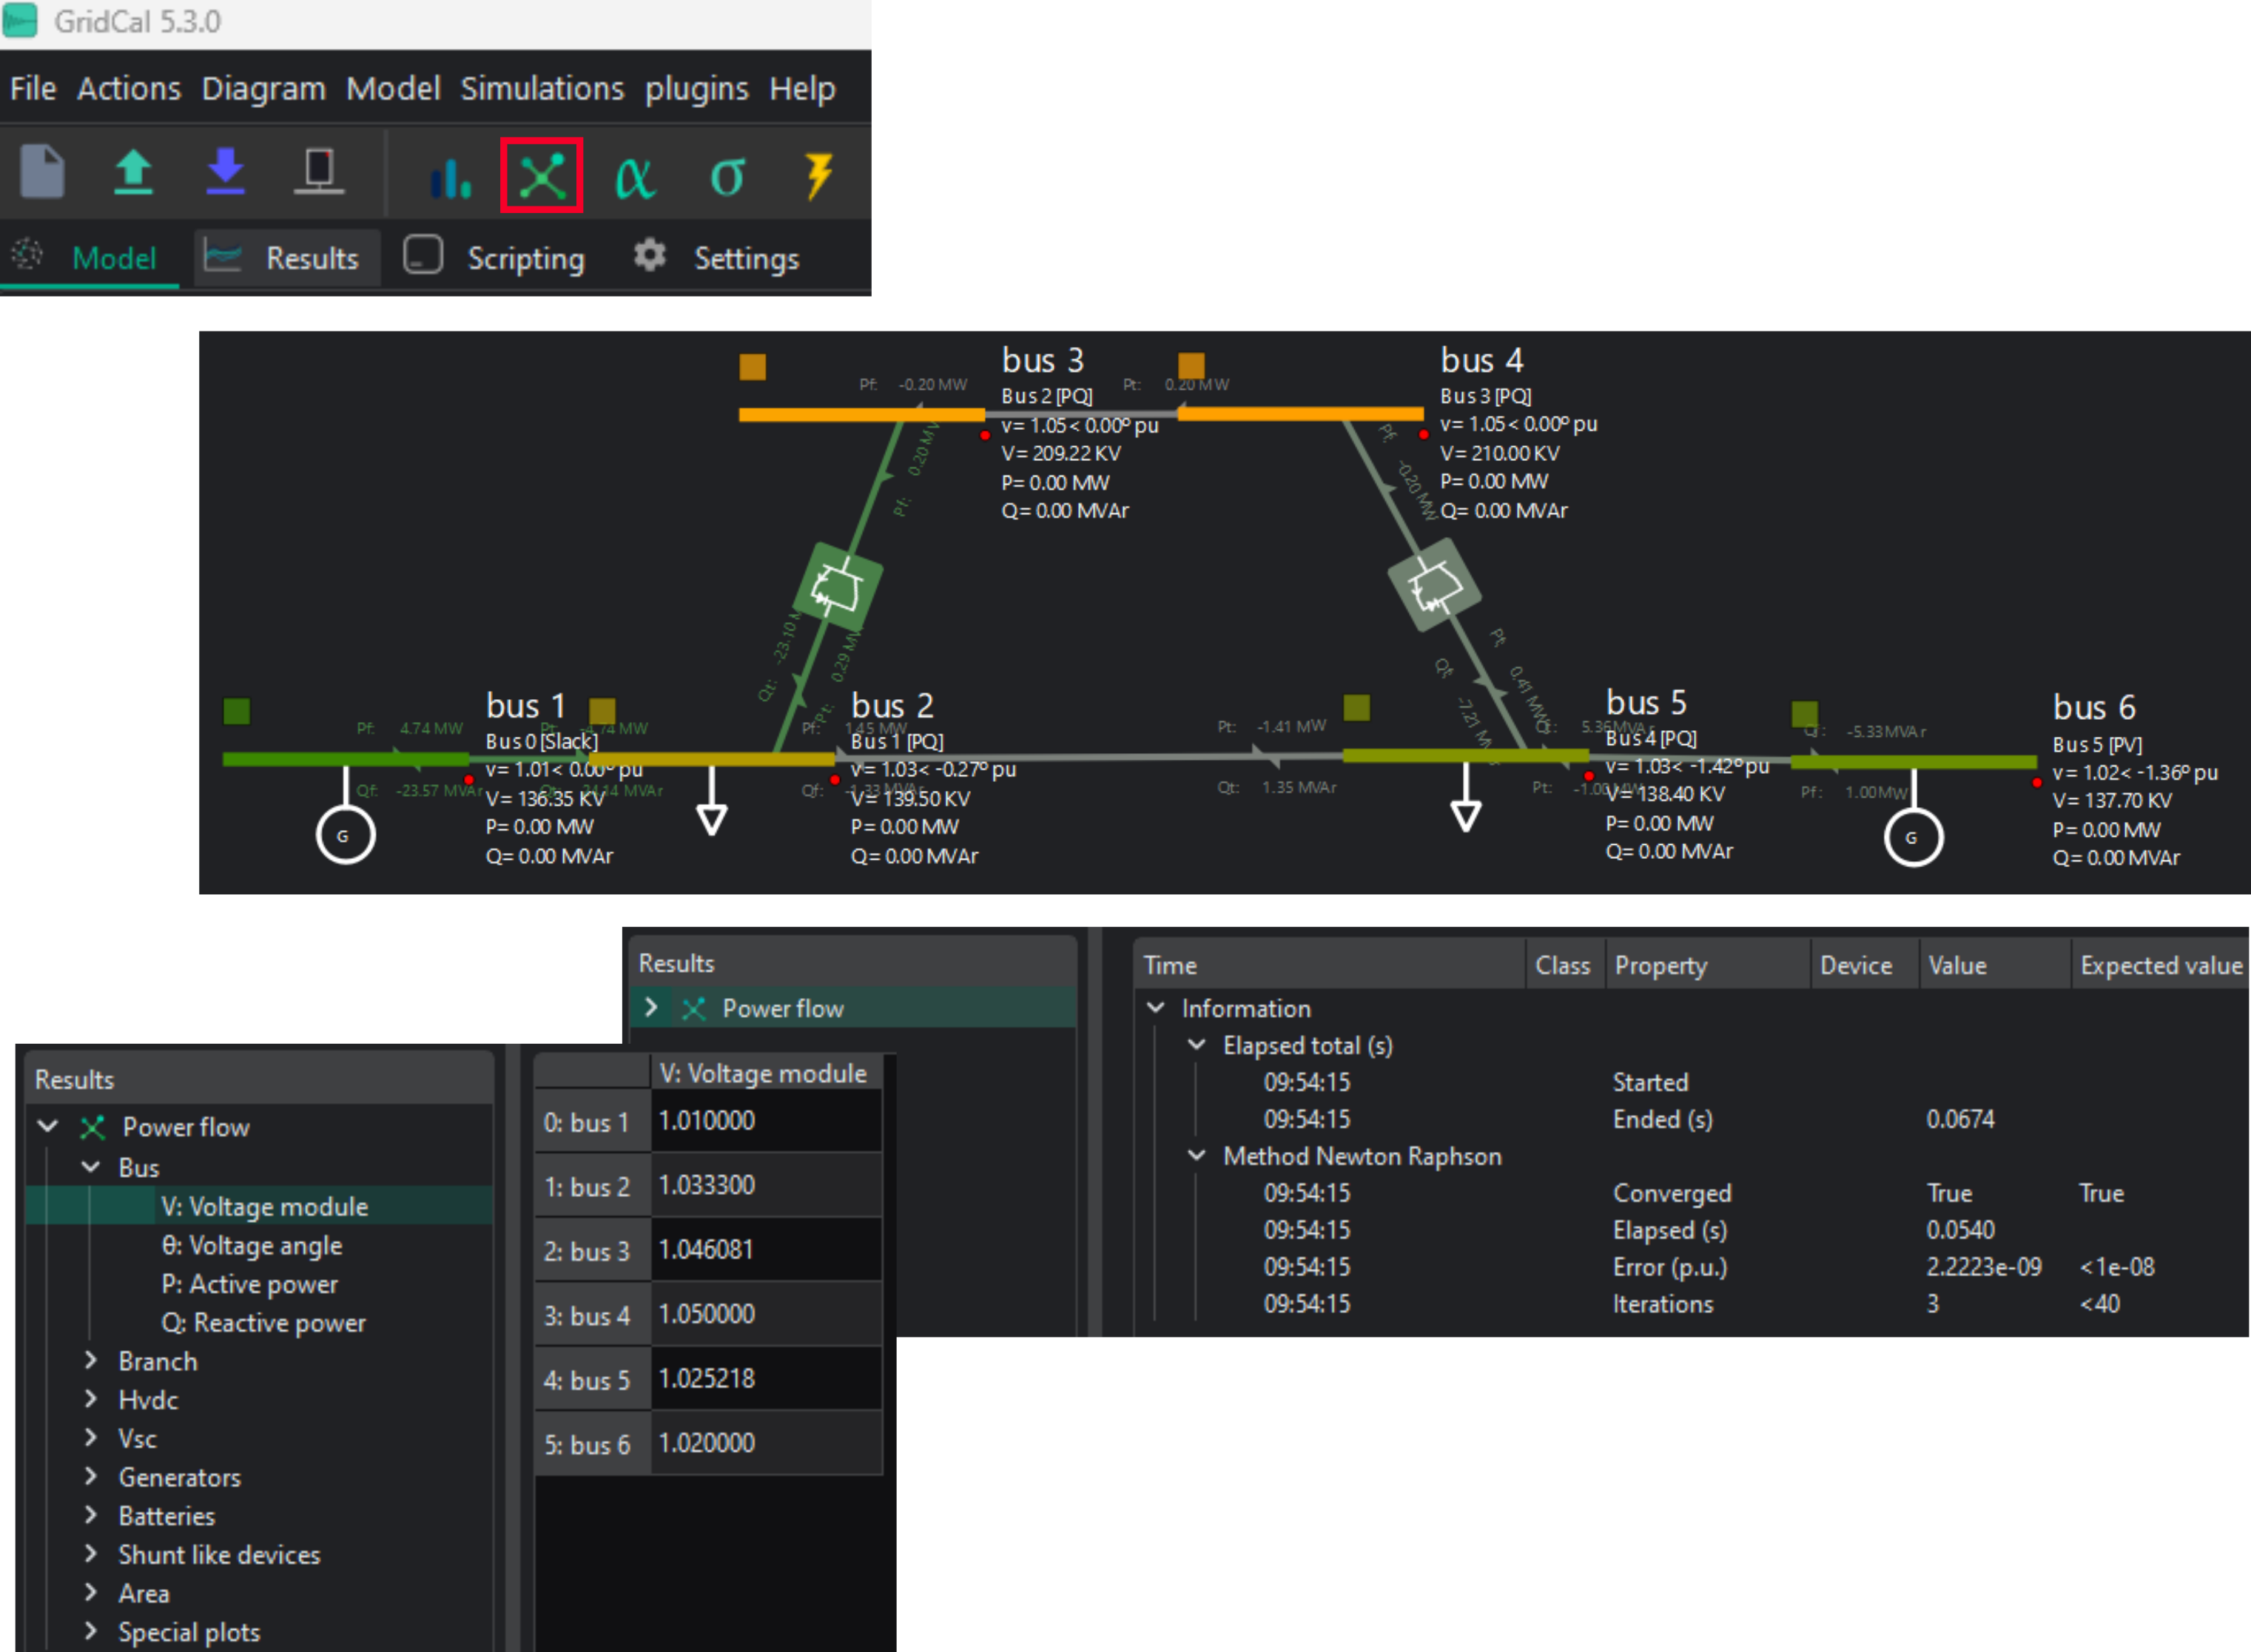
\includegraphics[width=0.75\textwidth]{Images/6busgui2.png}
    \caption{GUI simulation execution, solver selection and results visualization on the 6-bus grid.}
    \label{fig:6bus2}
    \end{figure}
\end{frame}

\begin{frame}{A few questions}
    Solver selection:
    \begin{itemize}
        \item Run the power flow with both the Newton-Raphson and the Gauss-Seidel.
        \item How many iterations do we need in both?
        \item What is the computational time?
    \end{itemize}
    Control setting:
    \begin{itemize}
        \item What if the two converters control active power?
        \item What if the two converters control voltage on the DC side?
    \end{itemize}
\end{frame}

\begin{frame}[fragile]{Scripting: modelling}
   % nothing, just work on the jupyter notebook 
   \begin{itemize}
    \item Let's move into our code editor.
   \end{itemize}

    \begin{lstlisting}[language=Python]
import numpy as np
import GridCalEngine as gce
from GridCalEngine.enumerations import ConverterControlType

# Grid instantiation
grid = gce.MultiCircuit()

# Define buses
bus1 = gce.Bus(name='B1', Vnom=135, is_slack=True)
...
    \end{lstlisting}
\end{frame}

\begin{frame}[fragile]{Scripting: solving}
   % nothing, just work on the jupyter notebook 
    \begin{itemize}
    \item Let's move into our code editor.
    \end{itemize}
    \begin{lstlisting}[language=Python]
pf_driver = gce.PowerFlowDriver(grid=grid)
pf_driver.run()
Vm = pf_driver.results.voltage
Va = np.angle(pf_driver.results.voltage, deg=True)
    \end{lstlisting}
\end{frame}

% ------------------------------------------
\subsection{Interconnected 17-bus case}
% \begin{frame}{}
%     \tableofcontents[currentsection]
% \end{frame}

\begin{frame}{Challenges of advanced cases}
    \begin{columns}
        
        \begin{column}{0.49\textwidth}
            \begin{itemize}
                \item The 6-bus case had 1 AC and 1 DC subsystem.
                \item Transnational grids are composed of many AC and DC grids.
                \item Real grids may also have controllable transformers.
            \end{itemize}
        \end{column}

        \begin{column}{0.5\textwidth}
            \begin{figure}[H]
                \centering
            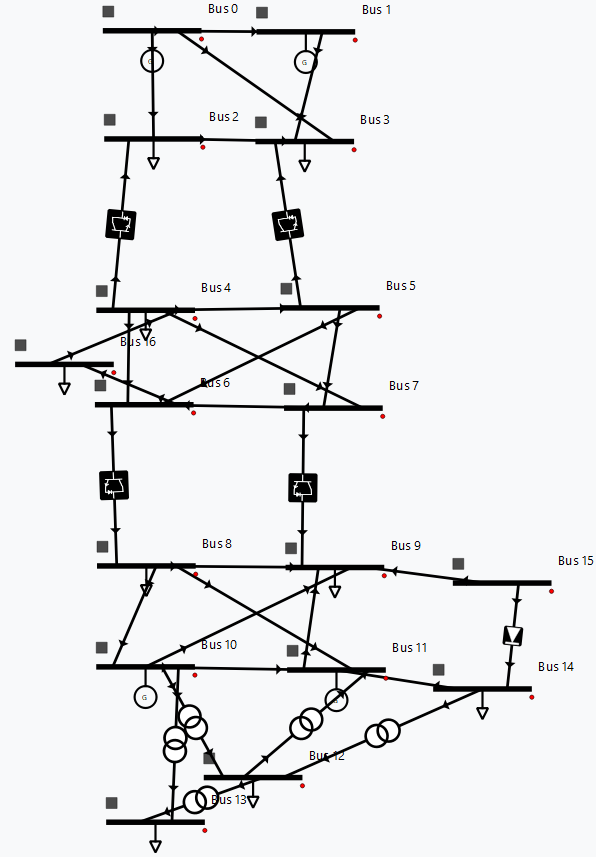
\includegraphics[width=0.73\textwidth]{Images/17busgui1.png}
            \caption{Interconnected AC systems overview.}
            \label{fig:17bus1}
            \end{figure}
        \end{column}

    \end{columns}

\end{frame}

\begin{frame}{Issues in the 17-bus cases}
    What issues are we facing?
    \begin{figure}[H]
        \centering
    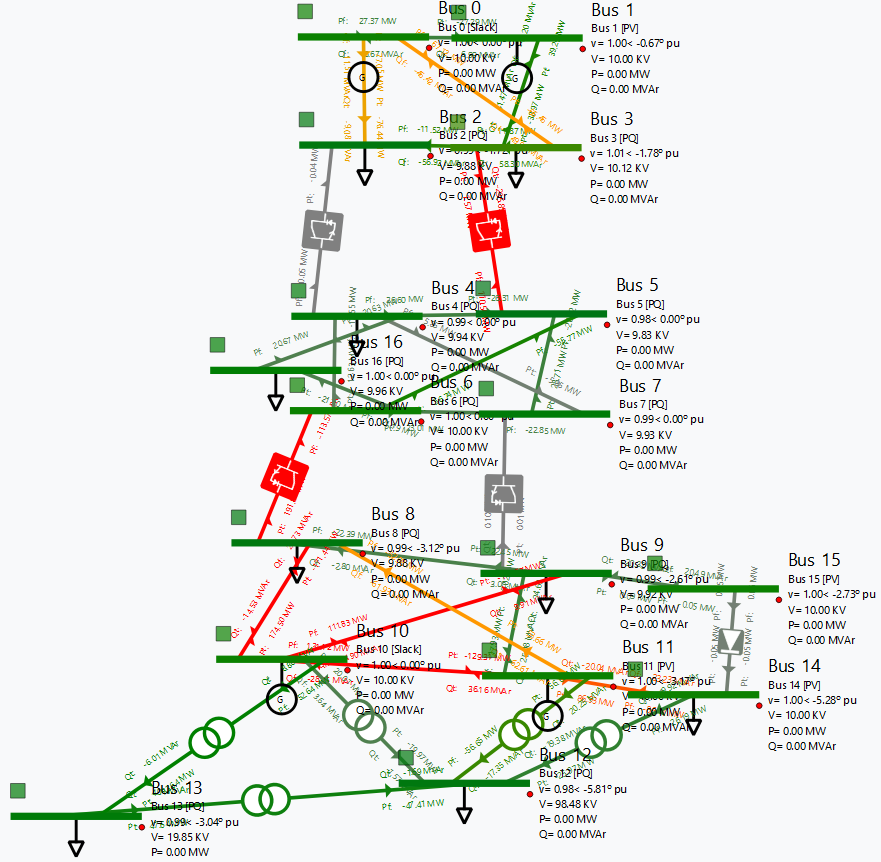
\includegraphics[width=0.52\textwidth]{Images/17bus_issues.png}
    \caption{Default interconnected AC system results.}
    \label{fig:17bus2}
    \end{figure}
\end{frame}

\begin{frame}{Fixing issues in the 17-bus cases}
    \begin{columns}
        
        \begin{column}{0.49\textwidth}
            Some potential fixes include:
            \begin{itemize}
                \item Adjust the transformer control setpoints.
                \item Change the VSCs control modes.
                \item Modify the VSCs control setpoints.
                \item Regulate the generators voltage reference.
            \end{itemize}
        \end{column}

        \begin{column}{0.5\textwidth}
            \begin{figure}[H]
                \centering
            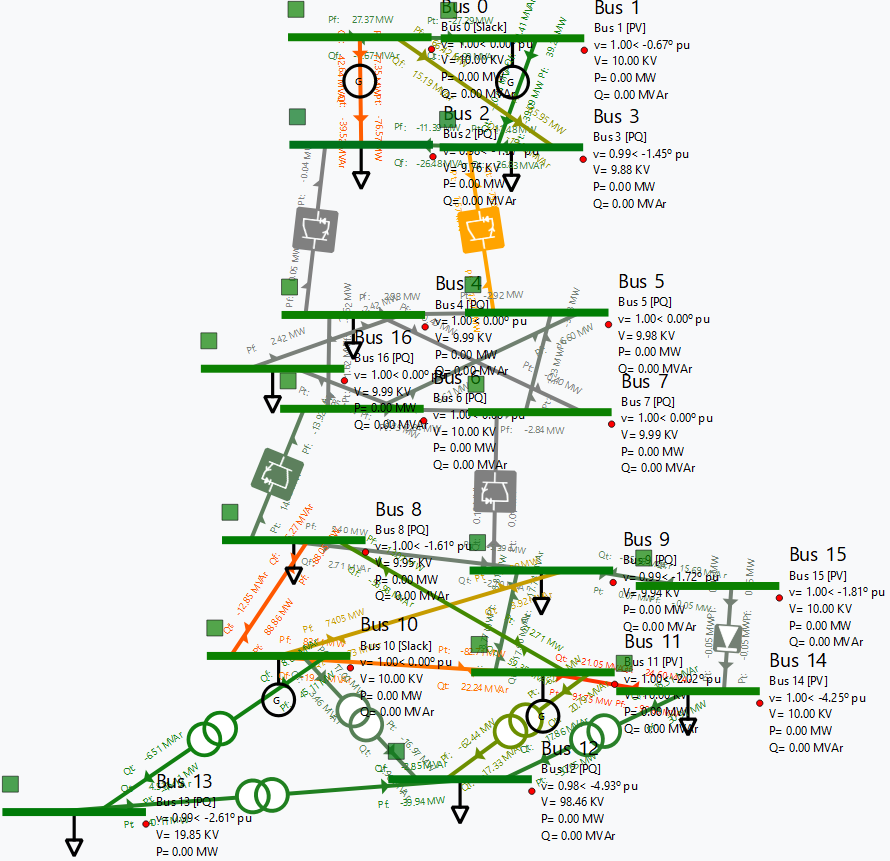
\includegraphics[width=0.93\textwidth]{Images/17bus_solved.png}
            \caption{Interconnected AC systems with a feasible solution.}
            \label{fig:17bus3}
            \end{figure}
        \end{column}
    \end{columns}
\end{frame}

\begin{frame}{Transformer control}

    \begin{columns}
        
        \begin{column}{0.5\textwidth}
    Despite being less flexible than VSCs, some transformers are also controllable:
    \begin{itemize}
        \item $m$: the tap module can regulate $V_m$ and $Q$
        \item $\tau$: the tap angle can adjust $P$
    \end{itemize}
    \begin{figure}[!htb]
        \centering
        \begin{circuitikz}[american]
            \draw[line width=0.7mm] (2,-1) to [short] (2,-2);
            \draw[line width=0.7mm] (7,-1) to [short] (7,-2);
            % \draw (2,-1.5) to [cute inductor, l=$m\angle \tau$] (7,-1.5);
            % \draw (2,-1.5) circle (0.3cm);
            % \draw (4.5,-1.5) circle (0.3cm);
            \draw (4.75,-1.5) circle (0.3cm);
            \draw (4.25,-1.5) circle (0.3cm);
            \node at (4.5,-1.0) {$m\angle \tau$};
            \draw (2,-1.5) to [short, i_=$P_f+jQ_f$]  (3.95,-1.5);
            \draw (7,-1.5) to [short, i=$P_t+jQ_t$]  (5.05,-1.5);
            \node at (2,-0.65) {$V_f \angle \delta_f$};
            \node at (7,-0.65) {$V_t \angle \delta_t$};
        \end{circuitikz}
        \caption{Representation of a controllable transformer.}
    \end{figure}
        \end{column}

        \begin{column}{0.5\textwidth}
            \begin{itemize}
            \item Let's increase $V_{m,13}$ to $1.019876$~p.u..
            \item Is it reasonable to have $0.9 \leq m \leq 1.0$?
            \end{itemize}
            \begin{figure}[H]
                \centering
            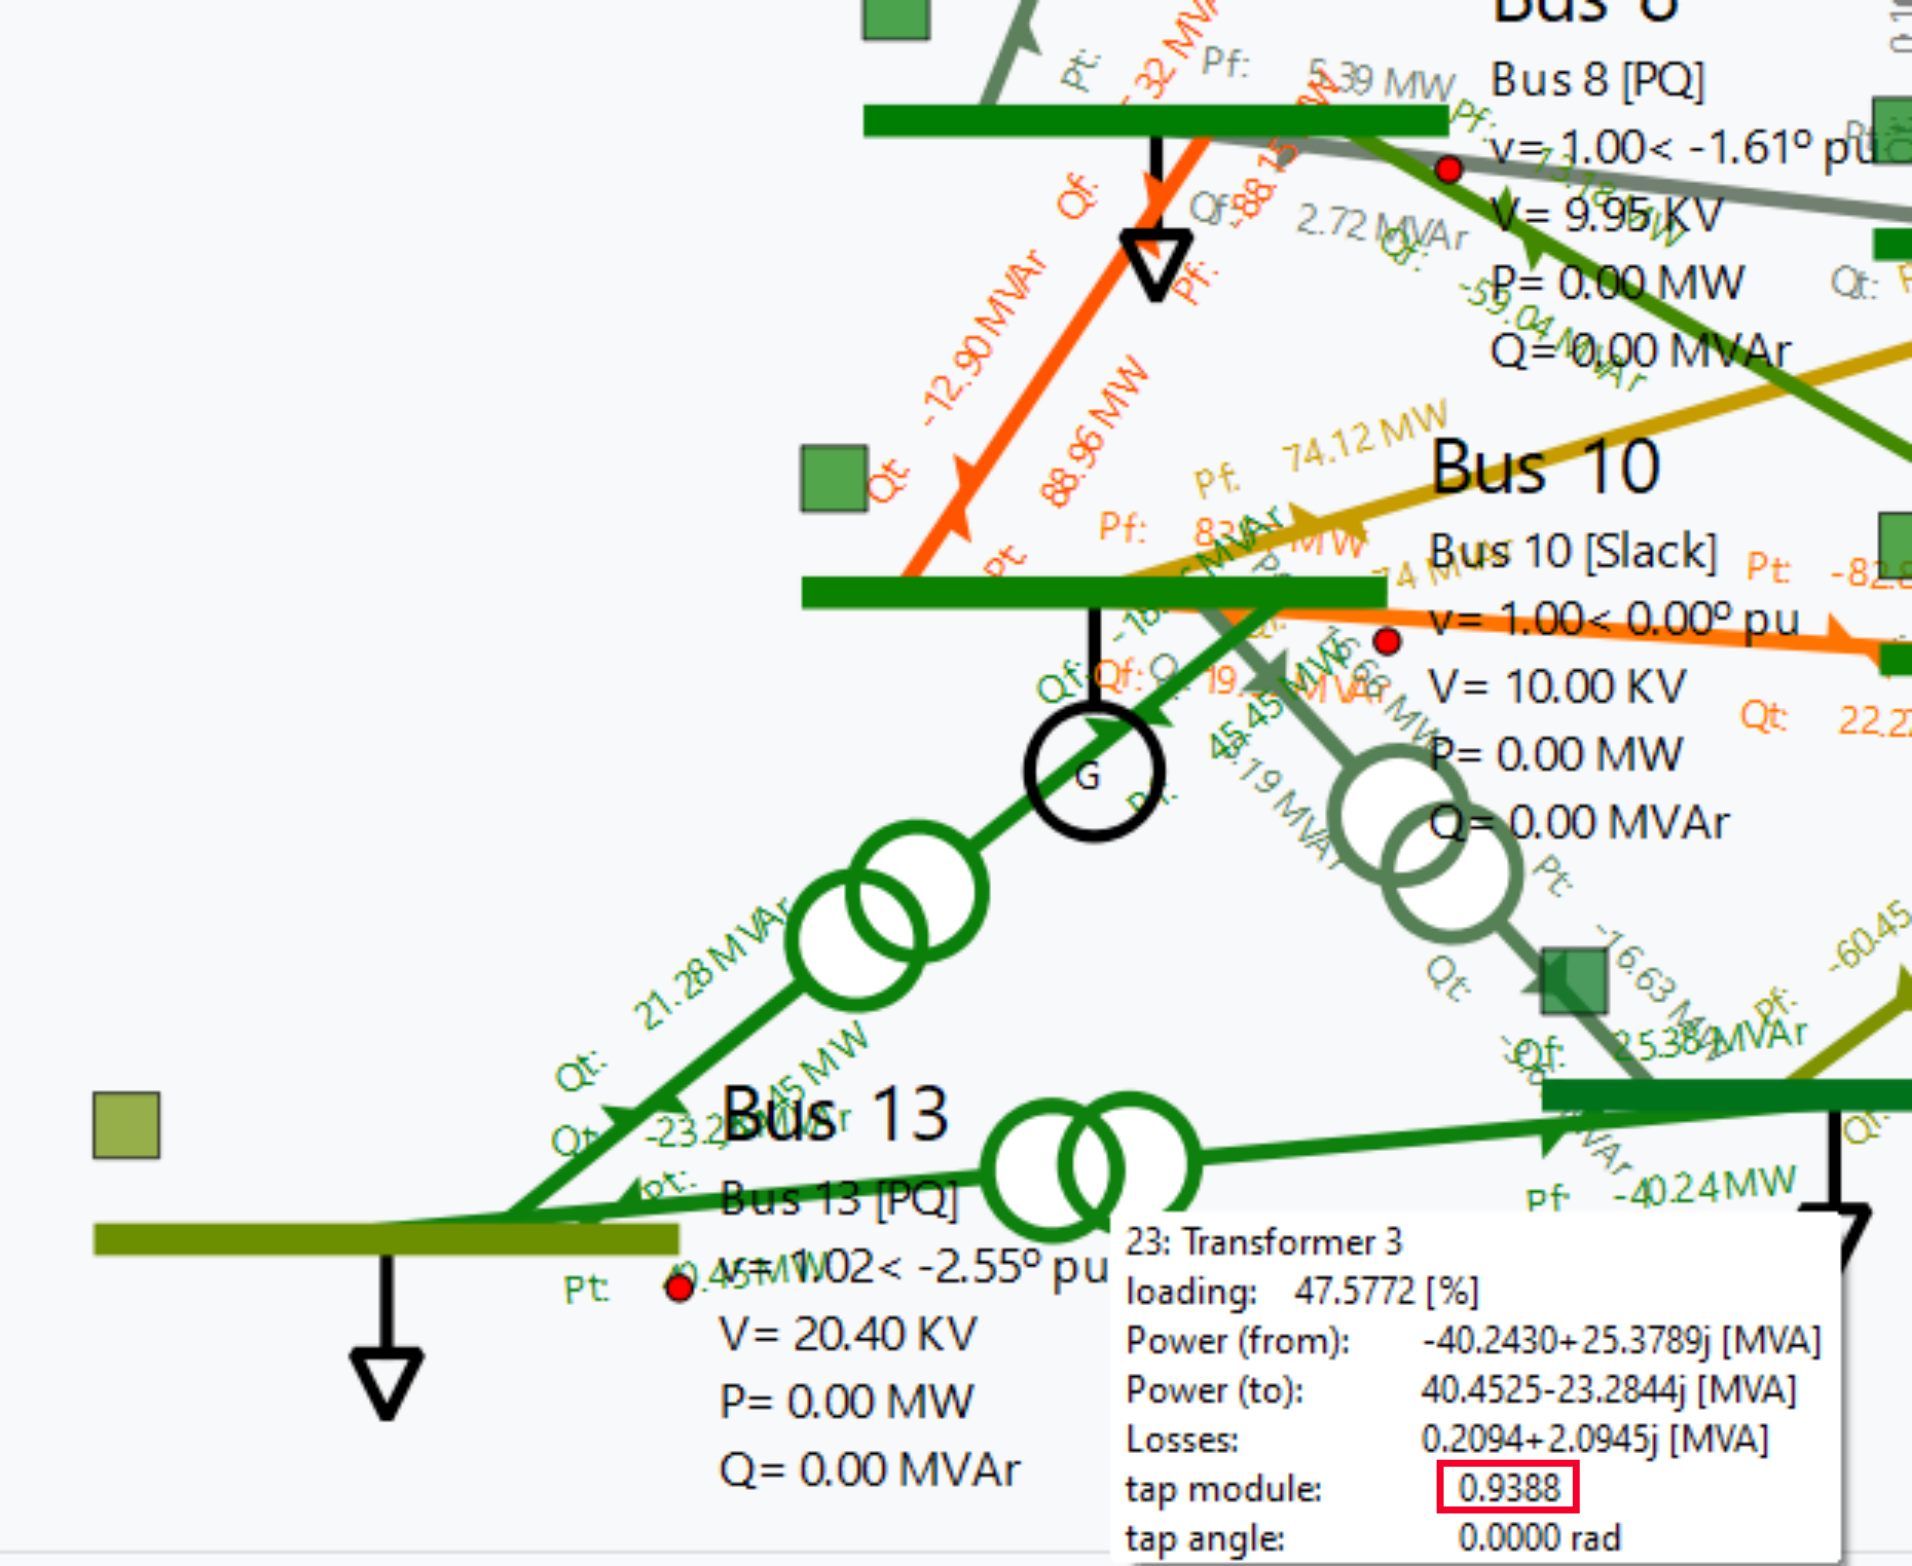
\includegraphics[width=0.85\textwidth]{Images/17bus_trafo.png}
            \caption{Transformer controlling $V_m$ with $m$.}
            \label{fig:17bus3}
            \end{figure}
        \end{column}
    \end{columns}
\end{frame}

% show how slow it goes with autodiff
% test setting some Va for grid-forming
% helm to get a feeling of solvability

% ------------------------------------------
\subsection{IEEE 118-bus case}
% first run HELM sigma and see we are getting some issues
% then add VSCs linking systems and show improvement in V profile

\begin{frame}{What is a large system?}
      \begin{figure}[H]
        \centering
    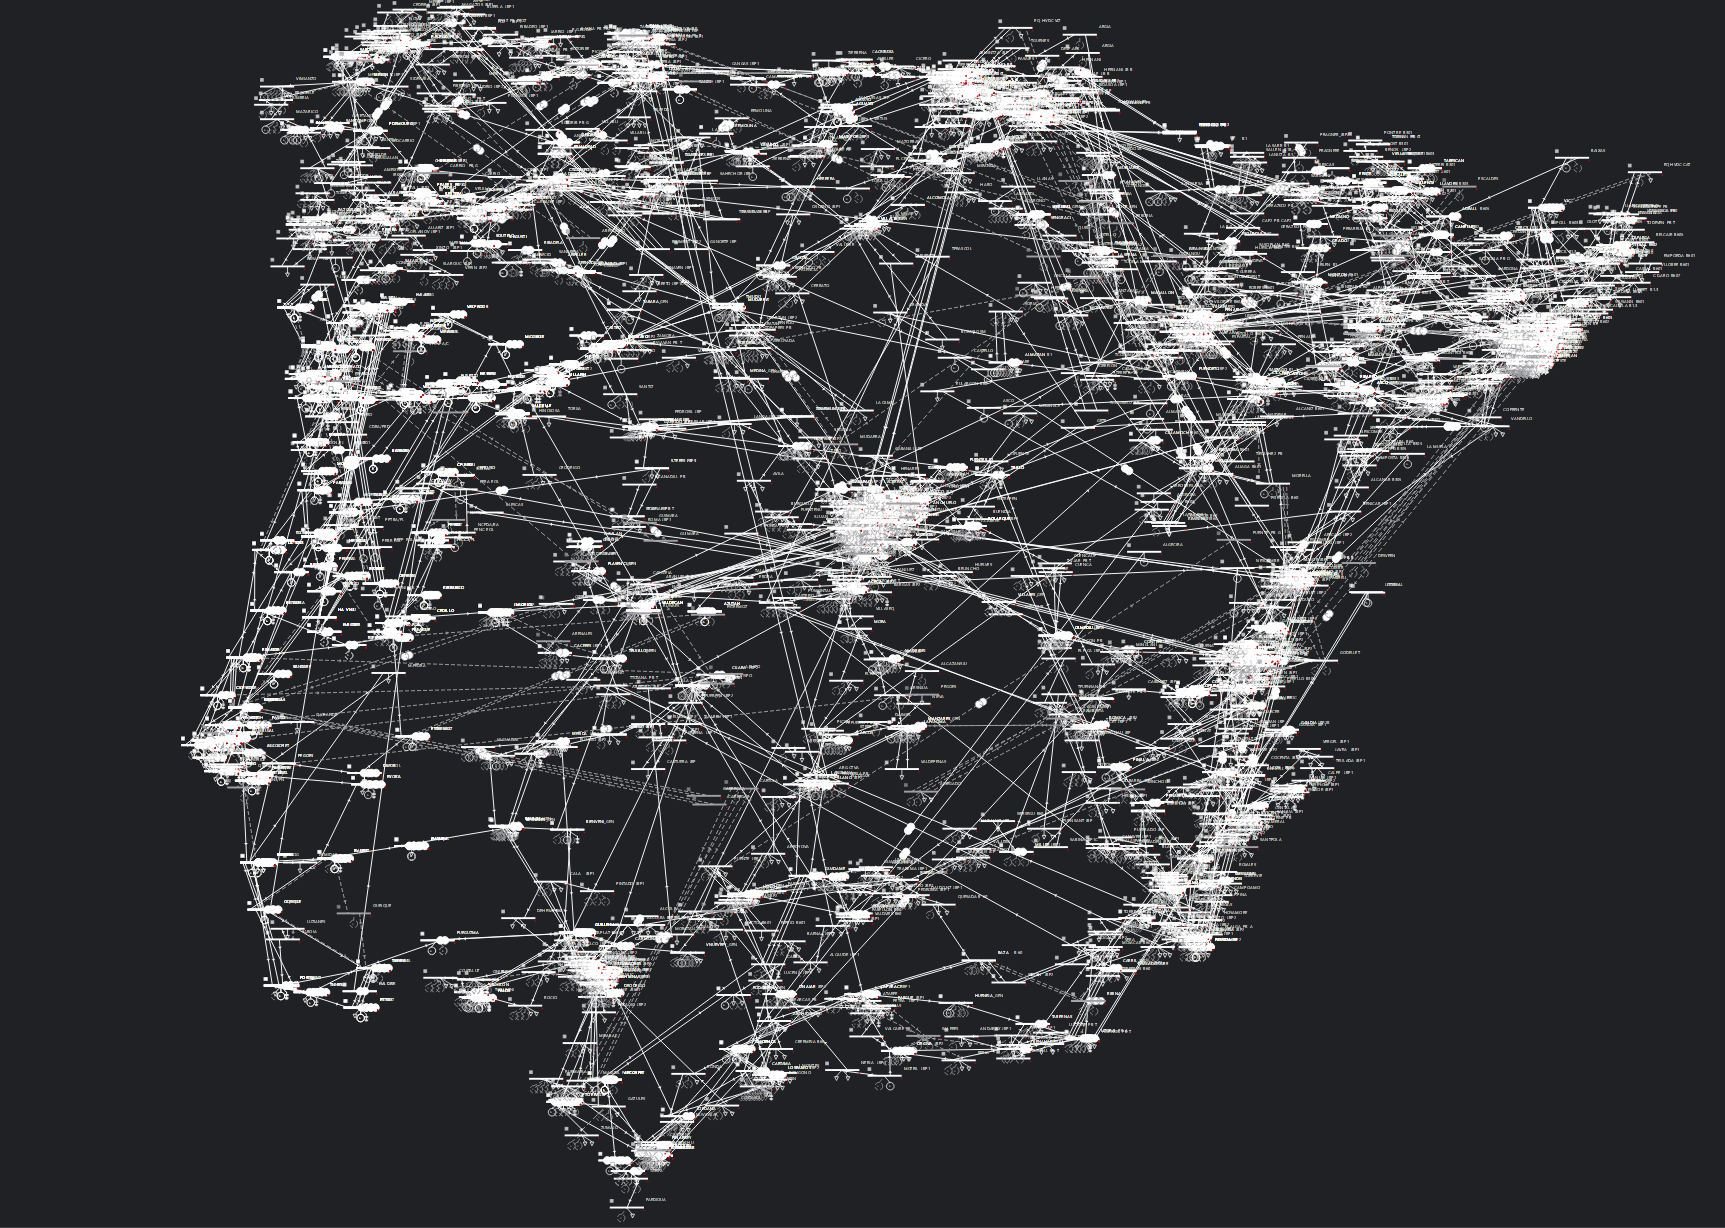
\includegraphics[width=0.75\textwidth]{Images/ESPgrid_topo.png}
    \caption{Grid topology of the Iberian system.}
    \label{fig:peninsula}
    \end{figure}   

\end{frame}

\begin{frame}{What is a large system?}
  \begin{itemize}
    \item Note: open the grid of Las Palmas to exemplify.
  \end{itemize} 
      \begin{figure}[H]
        \centering
    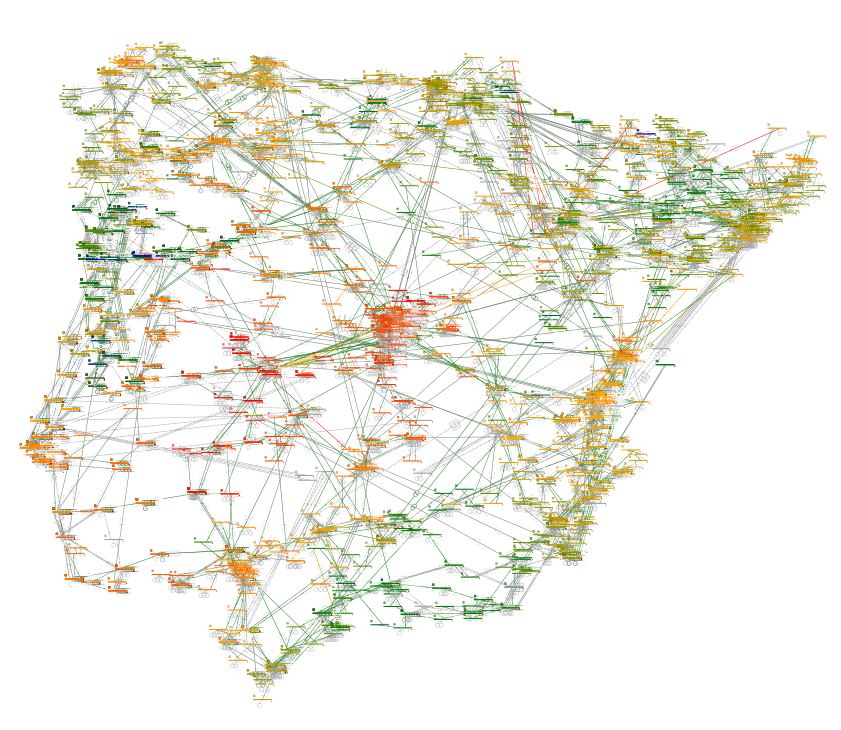
\includegraphics[width=0.60\textwidth]{Images/ESPgrid_solved.png}
    \caption{Solved power flow for the Iberian system.}
    \label{fig:peninsula2}
    \end{figure}   
\end{frame}

\begin{frame}{IEEE 118-bus operational overview}
    \begin{columns}
        
        \begin{column}{0.4\textwidth}
            \begin{itemize}
                \item Are voltage magnitudes correct?
                \item Are branch loadings within limits?
                \item How could an AC/DC link help?
            \end{itemize}
        \end{column}

        \begin{column}{0.45\textwidth}
     \begin{figure}[H]
        \centering
    % 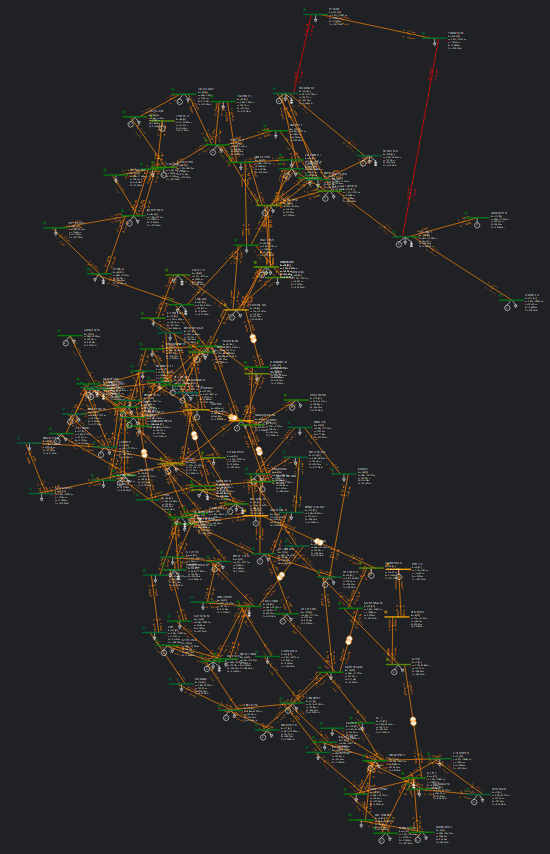
\includegraphics[width=0.65\textwidth]{Images/ie118_overscheme.png}
    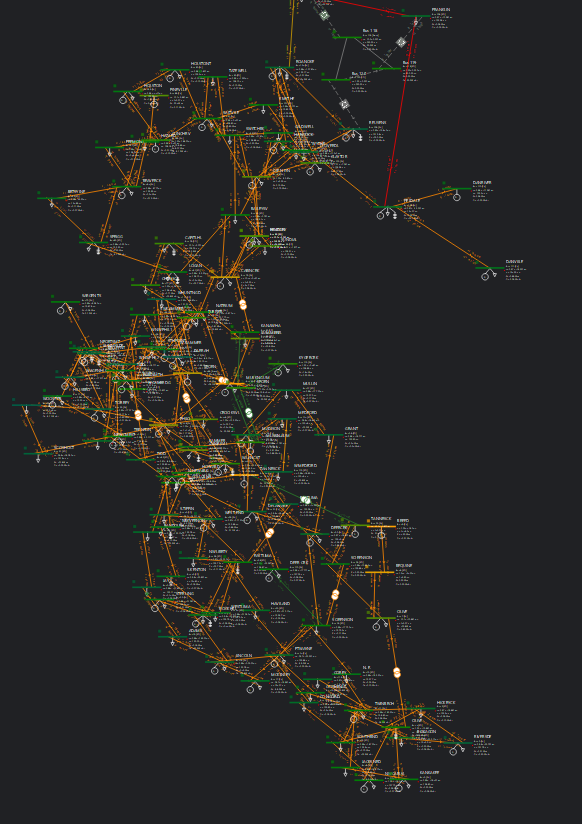
\includegraphics[width=0.80\textwidth]{Images/ie18_oper_v3.png}
    \caption{Original operation of the IEEE 118-bus grid.}
    \label{fig:118op}
    \end{figure}   
        \end{column}
    \end{columns}

\end{frame}

\begin{frame}{HELM analysis}
    \begin{figure}[H]
        \centering
    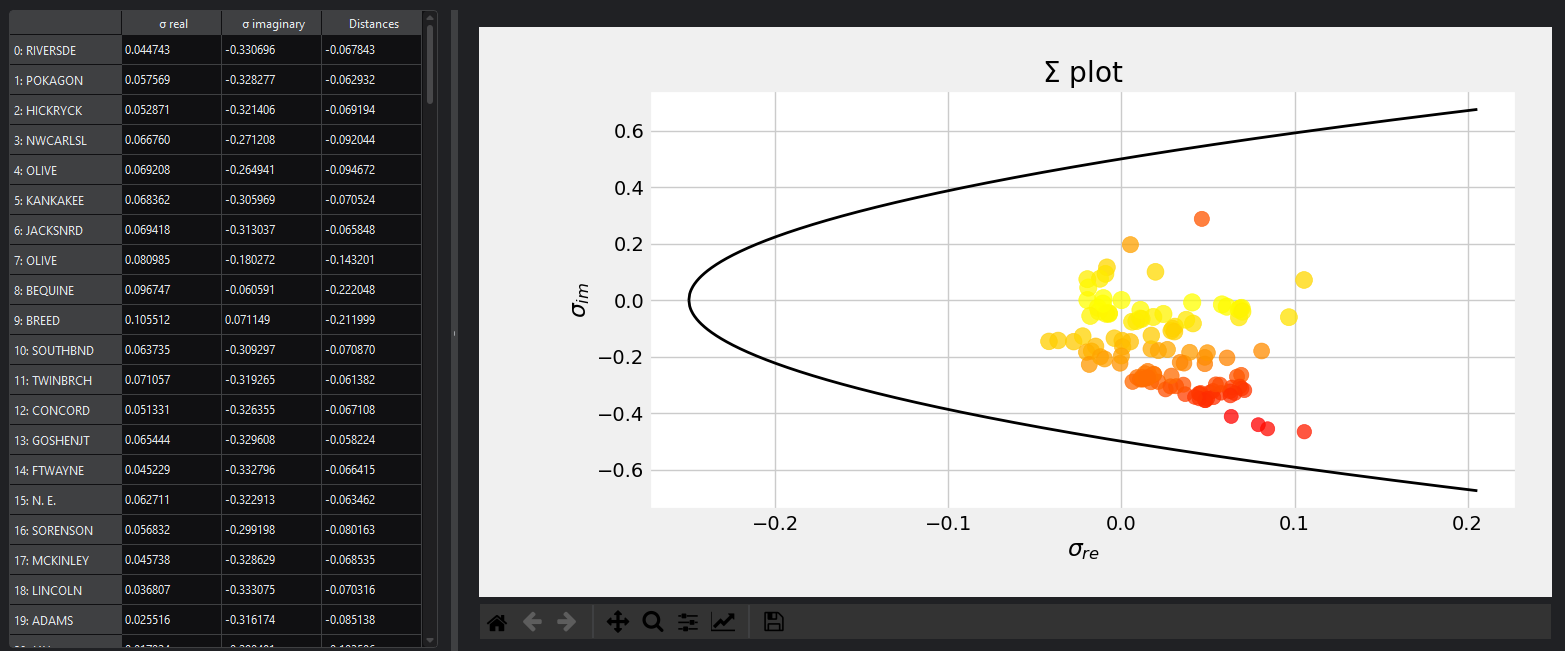
\includegraphics[width=0.99\textwidth]{Images/sigma_ie1182.png}
    \caption{HELM's Sigma plot showing showing the complicated feasibility of the systems.}
    \label{fig:118helm}
    \end{figure}
\end{frame}

\begin{frame}{Voltage and branch loading profiles}
    \begin{figure}[H]
        \centering
    % 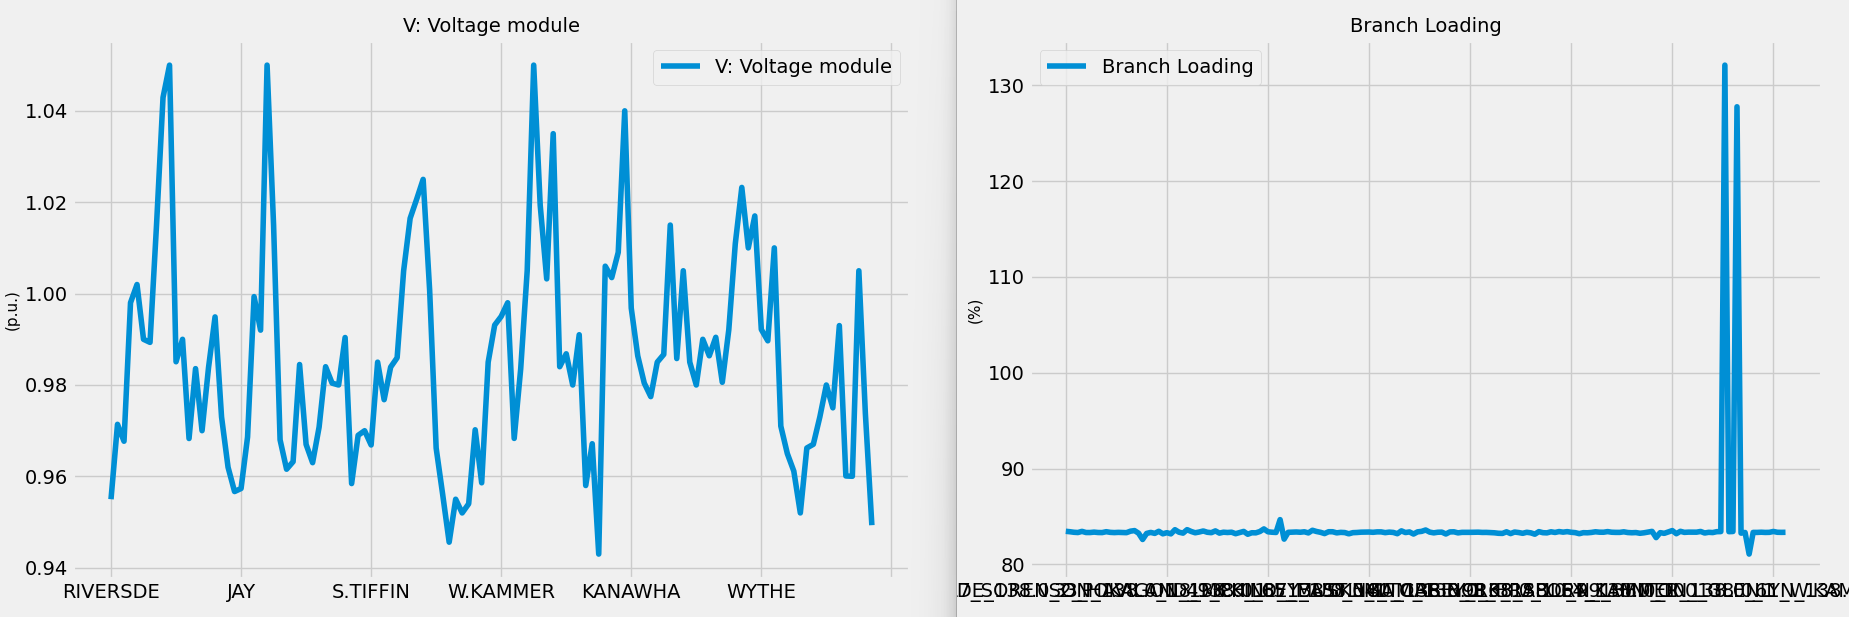
\includegraphics[width=0.99\textwidth]{Images/ie118_over.png}
    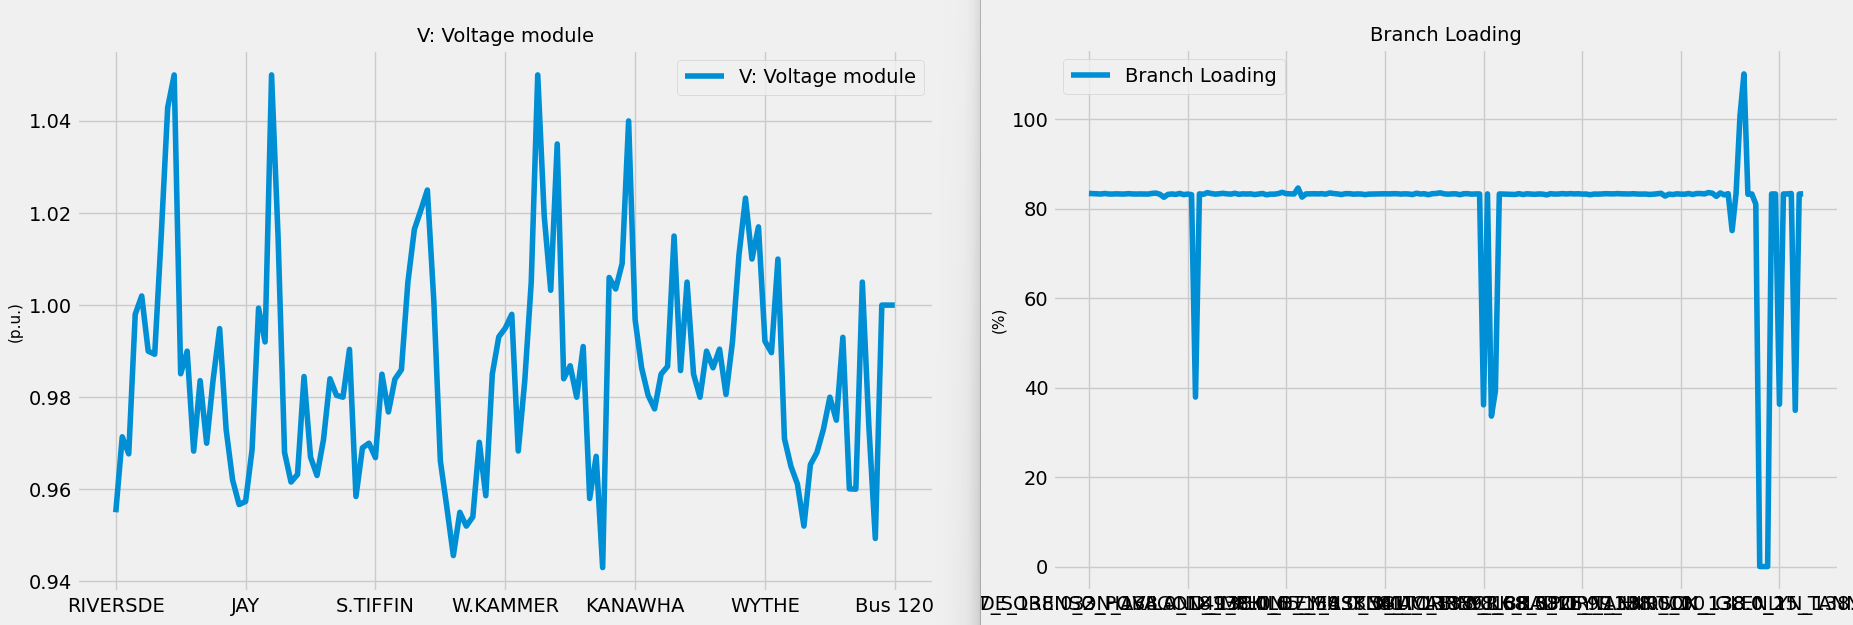
\includegraphics[width=0.99\textwidth]{Images/vl_ie18_v3.png}
    \caption{Voltage and branch loadings for the whole IEEE 118-bus system.}
    \label{fig:118vl}
    \end{figure}
\end{frame}

\begin{frame}{VSCs control management}
    \begin{figure}[H]
        \centering
    % 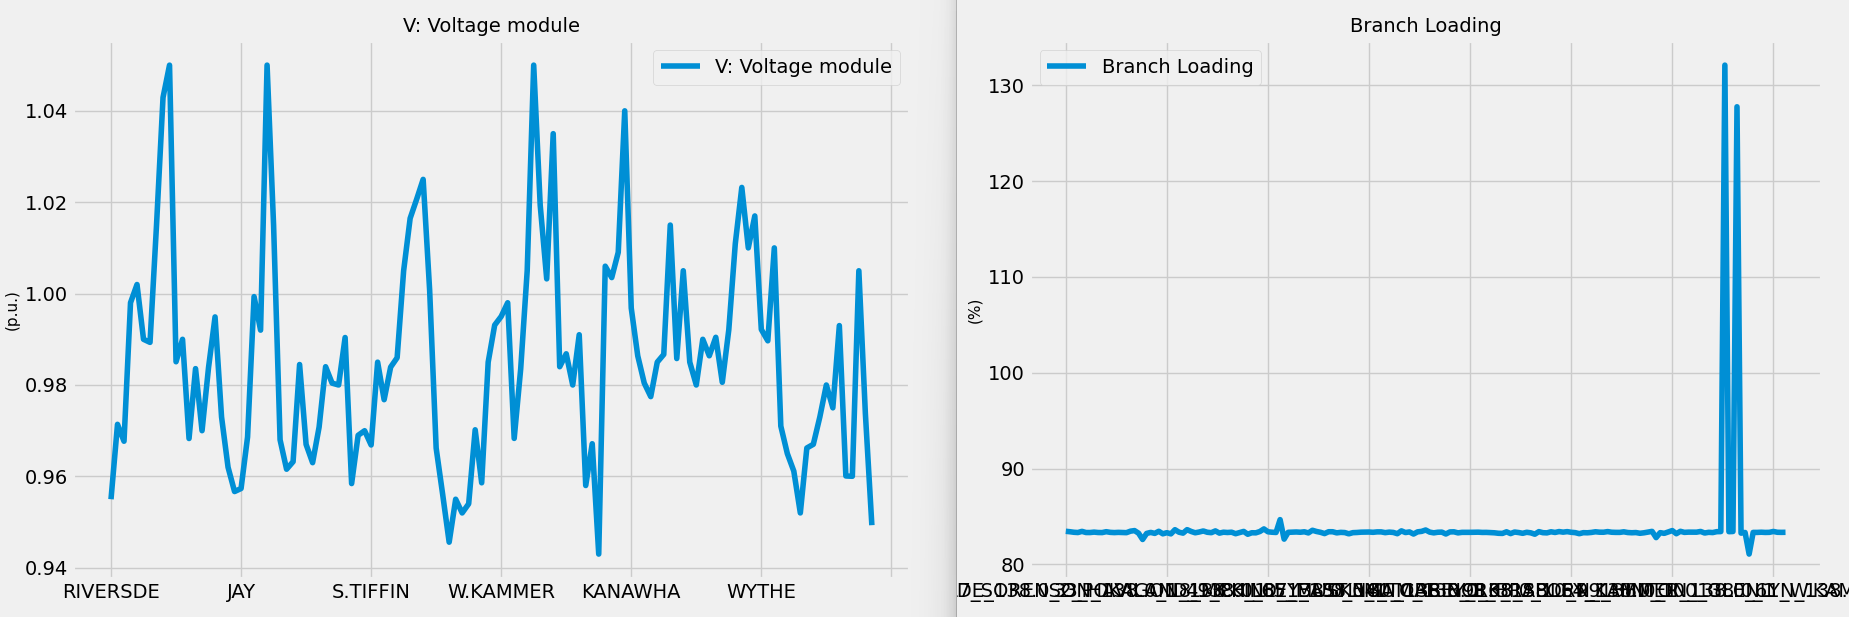
\includegraphics[width=0.99\textwidth]{Images/ie118_over.png}
    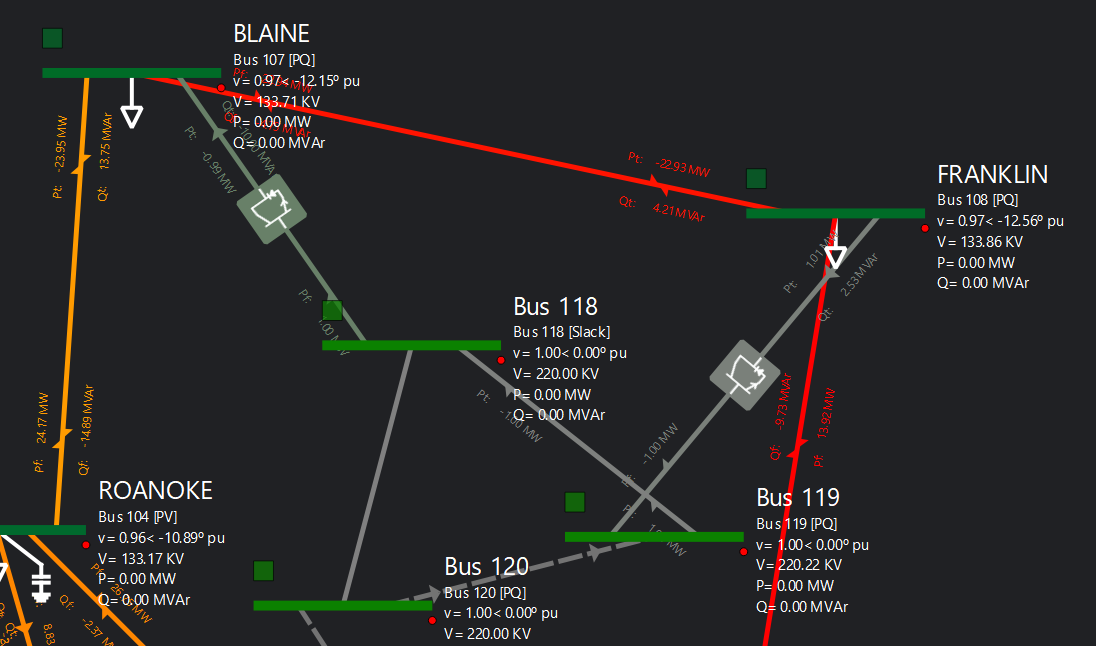
\includegraphics[width=0.90\textwidth]{Images/ie18_v3_fixed.png}
    \caption{Potential AC/DC link configuration.}
    \label{fig:118acdc}
    \end{figure}
\end{frame}






% \begin{frame}{}
%     \tableofcontents[currentsection]
% \end{frame}

% add some AC/DC vscs, show we solve it fast
% try the same with Gauss-Seidel and others. The way it is build should be straightfoward!?


% 5. Conclusions (just promote GridCal)
\section{Conclusions}

\begin{frame}{}
    \tableofcontents[currentsection]
\end{frame}

\begin{frame}{Conclusions}
    \begin{itemize}
        \item AC/DC converters require a new approach to their modelling.
        \item The Newton-Raphson method is the go-to algorithm due to its convergence properties.
        \item Setting the right AC/DC controls is key towards achieving a convergent case.
        \item Importance of relying on a GUI.
    \end{itemize}
    
\end{frame}


\begin{frame}[plain]
\hspace*{-1.0cm}\parbox[t]{\textwidth}{
	\titlepage
    } 
\end{frame}

% \begin{frame}{Environmental, Social, and Gender Impact}
%     \begin{itemize}
%         \item \textbf{Environmental Impact}: 
%         The algorithm improves renewable energy integration, facilitating wind and solar power integration, which is crucial for reducing greenhouse gas emissions.
        
%         \item \textbf{Social Impact}: 
%         Increased efficiency leads to reduced operational costs, which can lower electricity prices, improving access to reliable power and reducing energy poverty in developing regions.
        
%         \item \textbf{Gender Impact}: 
%         By lowering household energy costs, the algorithm alleviates financial burdens that disproportionately affect women, especially in energy-poor regions. It also creates more equitable opportunities by improving energy access for education, healthcare, and economic participation.
%     \end{itemize}
% \end{frame}


% \begin{frame}{Time Planning}
%     The time spent on this project is broken down in the chart below. Many tasks were performed in parallel, and at times going back and forth between different processes.

%     \begin{figure}[htbp]
%         \centering
%         \begin{ganttchart}[
%             vgrid={*{32}{draw=none}, dotted},
%             hgrid,
%             title/.append style={fill=none},
%             title label font=\bfseries\footnotesize,
%             title label anchor/.append style={below=-1.6ex},
%             include title in canvas=false,
%             bar/.append style={fill=gray!30},
%             bar label font=\small\sf,
%             bar label node/.append style={left=3pt},
%             bar incomplete/.append style={fill=gray},
%             x unit=0.3cm, % Decreased width
%             y unit title=0.5cm,
%             y unit chart=0.6cm
%         ]{1}{32}  % 32 blocks representing a finer division
%             % Months title (each multiplied by 4)
%             \gantttitle{2024}{32} \\
%             \gantttitle{Jan}{4}
%             \gantttitle{Feb}{4}
%             \gantttitle{Mar}{4}
%             \gantttitle{Apr}{4}
%             \gantttitle{May}{4}
%             \gantttitle{Jun}{4}
%             \gantttitle{Jul}{4}
%             \gantttitle{Aug}{4} \\
%             % Tasks
%             \ganttbar{Literature Review}{6}{12} \\
%             \ganttbar{Model Development}{8}{20} \\
%             \ganttbar{Model Validation}{16}{24} \\
%             \ganttbar{GridCal Prototype}{20}{28} \\
%             \ganttbar{Benchmarking}{28}{30} \\
%             \ganttbar{Documentation}{30}{32}  % Ending at the 32nd block
%         \end{ganttchart}
%         \caption{Gantt Chart for the project.}
%     \end{figure}
% \end{frame}

% \begin{frame}{Budget}
%     In the table below, we see the costs associated with the project. The project was done in conjunction with eRoots Analytics SL, over a period of 24 weeks. These hours were split between the development engineer and the supervisor.

%     \begin{table}[H]
%         \centering
%         \caption{Costs of the project.}
%         \label{tab:costs}
%         \begin{tabular}{|l|c|c|c|}
%         \hline
%         \textbf{Role} & \textbf{Hours} & \textbf{Hourly Rate (€)} & \textbf{Total Cost (€)} \\ \hline
%         Development Engineer & 520 & 50 & 26.000 \\ \hline
%         Supervisor & 260 & 60 & 15.600 \\ \hline
%         \textbf{Total} & \textbf{780} & \textbf{} & \textbf{41.600} \\ \hline
%         \end{tabular}
%     \end{table}
%     The total cost of the project was € 41.600.
% \end{frame}


% \begin{frame}{Depth-First Search (DFS)}
%     \begin{figure}[H]
%         \centering
%         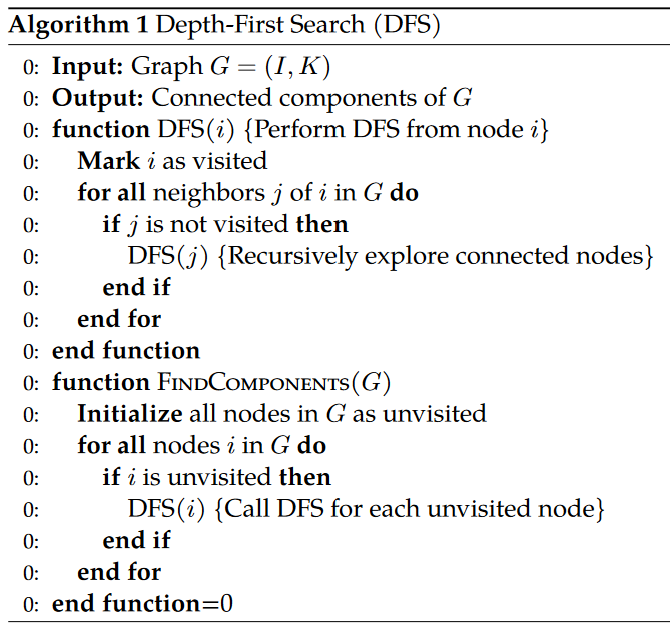
\includegraphics[width=0.8\textwidth]{chapter5pics/dfs.png}
%         \caption{Depth-First Search (DFS) algorithm.}
%         \label{fig:dfs}
%     \end{figure}
% \end{frame}




\end{document}

